\documentclass[11pt,letterpaper]{article}
\usepackage[margin=1in]{geometry}
\usepackage[T1]{fontenc}
\usepackage{lmodern}
\usepackage{amsmath,amssymb,mathtools,bm,slashed}
\usepackage{microtype,graphicx,booktabs,array}
\usepackage[numbers,sort&compress]{natbib}
\usepackage[colorlinks=true,linkcolor=blue,citecolor=blue,urlcolor=blue]{hyperref}
\usepackage[nameinlink,noabbrev]{cleveref}
\numberwithin{equation}{section}
\newcommand{\dd}{\mathrm d}
\newcommand{\MeV}{\mathrm{MeV}}
\newcommand{\CK}{\mathcal C_K}
\newcommand{\Izero}{\mathcal I_0}
\newcommand{\Jtwo}{\mathcal J_2}
\newcommand{\pos}[1]{\left[#1\right]_+}
\DeclareMathOperator{\sech}{sech}
\title{The Nonleptonic Weak Rate in Massless Quark Matter:\\Exact Cold Phase Space and the Thermal Correction Through \(T^2\)}
\author{Standalone derivation and numerical verification}
\date{October 11, 2026}

\begin{document}
\maketitle
\begin{abstract}
We derive the net rate of \(d+u\leftrightarrow s+u\) for massless quarks with unequal flavor chemical potentials.
Starting from the invariant collision integral, we reduce the finite-temperature rate to two numerical integrations and obtain the exact cold rate for the ordering selected by charge-neutral, electron-free matter.
The cold phase space has two branches separated by \(\mu_d-\mu_s=\mu_u\).
We derive the order-\(T^2\) correction by expanding the four occupation factors independently and distinguish it from the additional chemical-potential shifts imposed by neutrality at fixed \(\mu_B,\mu_K\).
The coincident incoming and outgoing up-quark thresholds generate a cubic thermal remainder, which we also derive and test.
The nearly equal-flavor limit recovers the familiar cubic-plus-thermal-linear rate, but that limit is not imposed in the general result.
Symbolic identities and numerical phase-space calculations test the normalization, branch matching, limiting cases, and accuracy of the temperature truncation.
We also compare rate-integral speed estimates at fixed isothermal backgrounds and along conserved adiabatic EOS trajectories reconstructed from upstream neutron matter.
The calculation includes the tree-level four-quark channel only; it does not include strong-interaction corrections or additional antiquark reactions.
\end{abstract}

\section{Physical rate and conventions}
\label{sec:conventions}
We consider unpaired, massless quarks in local kinetic equilibrium at a common temperature \(T\), with independent flavor chemical potentials \(\mu_u,\mu_d,\mu_s\).
Natural units \(\hbar=c=k_B=1\) and the metric \(g^{\mu\nu}=\operatorname{diag}(1,-1,-1,-1)\) are used throughout.
The reaction and sign convention are
\begin{equation}
 d(p_d)+u(p_1)\longleftrightarrow s(p_s)+u(p_2),
 \qquad \mu_K=\mu_d-\mu_s,
 \qquad n_K=\frac{n_d-n_s}{2}.
 \label{eq:reaction}
\end{equation}
A forward event decreases \(n_K\) by one unit, so the positive relaxation source is
\begin{equation}
 \Gamma_K=R(d+u\to s+u)-R(s+u\to d+u),
 \qquad \left.\frac{\dd n_K}{\dd t}\right|_{\rm reactions}=-\Gamma_K.
 \label{eq:source}
\end{equation}
The baryon and imbalance chemical potentials satisfy
\begin{equation}
 \mu_B=\mu_u+\mu_d+\mu_s,
 \qquad \mu_K=\mu_d-\mu_s.
 \label{eq:chemical-basis}
\end{equation}
Quark charge neutrality without electrons gives \(2n_u=n_d+n_s\).
For the massless equation of state,
\begin{equation}
 n_f=\frac{\mu_f^3}{\pi^2}+\mu_fT^2,
 \quad n_u=n_B,\quad n_d=n_B(1+a),\quad n_s=n_B(1-a),
 \label{eq:density}
\end{equation}
and monotonicity of \(n_f(\mu_f,T)\) implies
\begin{equation}
 0\leq\mu_s<\mu_u<\mu_d\qquad (0<a\leq1).
 \label{eq:ordering}
\end{equation}
The equilibrium limit \(a=0\) is taken by continuity.

The interaction and normalization follow Madsen~\cite{Madsen:1993xx}, with the down and strange labels exchanged relative to his forward reaction.
Both of his printed cold branches, Eqs.~(20) and (21), require \(\mu_u<\mu_d\) in his labeling.
After reversing the reaction, that condition would require \(\mu_u<\mu_s\), contrary to \cref{eq:ordering}.
The cold expressions below are therefore obtained from the collision integral rather than by extending those formulas beyond their stated domains.
This calculation retains the weak interaction at tree level and omits quark masses, QCD corrections to the matrix element and dispersion relations, pairing, and additional channels containing antiquarks.
The massless density in \cref{eq:density} is a net density, whereas the collision integral below counts the stated quark channel; using the exact density does not supply the omitted antiquark reaction channels at high temperature.

\section{Invariant collision integral}
\label{sec:invariant}
For each leg, let \(p_i^\mu=(E_i,\bm p_i)\), with \(E_i=|\bm p_i|\), and define
\begin{equation}
 f_f(E)=\frac{1}{1+\exp[(E-\mu_f)/T]}.
 \label{eq:fermi}
\end{equation}
Using Madsen's matrix element [Eq.~(5)] and spin--color convention with the standard invariant phase-space measure, the forward rate per unit volume and time is\footnote{Madsen's Eq.~(4) prints \((2\pi)^{-5}\) multiplying the bare momentum measures, whereas the standard invariant measure gives \((2\pi)^{-8}\).
The printed factor is a normalization misprint: \((2\pi)^{-8}\) is consistent with his Eqs.~(13) and (20)--(22) and with the calculation in \cref{app:normalization}.}
\begin{align}
 R(d+u\to s+u)
 &=\frac{36}{2}\int\prod_{i=1,d,2,s}
 \frac{\dd^3\bm p_i}{(2\pi)^3\,2E_i}
 (2\pi)^4\delta^{(4)}(p_1+p_d-p_2-p_s)
 |\mathcal M|^2\notag\\
 &\hspace{28mm}\times f_u(E_1)f_d(E_d)
 [1-f_u(E_2)][1-f_s(E_s)],
 \label{eq:invariant-rate}\\
 |\mathcal M|^2
 &=64G_F^2\sin^2\theta_C\cos^2\theta_C
 (p_1\cdot p_d)(p_2\cdot p_s).
 \label{eq:matrix}
\end{align}
The combined factor in \cref{eq:invariant-rate,eq:matrix} can be derived without any spin-average convention from
\begin{equation}
 \mathcal H_{\rm eff}=\frac{G_F}{\sqrt2}\sin\theta_C\cos\theta_C
 [\bar u\gamma^\alpha(1-\gamma^5)d]
 [\bar s\gamma_\alpha(1-\gamma^5)u]+\text{h.c.}
 \label{eq:interaction}
\end{equation}
Summing all four external spins gives \(128G_F^2\sin^2\theta_C\cos^2\theta_C(p_1\cdot p_d)(p_2\cdot p_s)\), as shown by the traces in \cref{app:normalization}.
The color-singlet currents preserve color along each fermion line, leaving \(3\times3=9\) color choices.
Their product is \(9\times128=1152=(36/2)\times64\), exactly the combined normalization in Madsen's convention.
His factor \(36\) counts incoming spin--color states and his separate \(1/2\) accounts for the incoming up-quark helicity; the quoted matrix element and these factors must be used together.
The two up legs are on opposite sides of the reaction, so there is no additional identical-particle factorial.
Recovery of the equal-flavor rate below supplies a second normalization check.

The identity \(f_f/(1-f_f)=\exp[(\mu_f-E)/T]\), together with energy conservation, gives
\begin{equation}
 \frac{f_u(E_2)f_s(E_s)[1-f_u(E_1)][1-f_d(E_d)]}
 {f_u(E_1)f_d(E_d)[1-f_u(E_2)][1-f_s(E_s)]}
 =e^{-\mu_K/T}.
 \label{eq:balance-ratio}
\end{equation}
Consequently,
\begin{equation}
 \Gamma_K=(1-e^{-\mu_K/T})R(d+u\to s+u)
 \qquad (T>0).
 \label{eq:detailed-balance}
\end{equation}
For \(\mu_K>0\), the rate is positive and the reverse process is exponentially small as \(T\to0\) at fixed nonzero \(\mu_K\).
At equilibrium the net rate vanishes even though both one-way rates are nonzero at finite temperature.
Numerical evaluation of the prefactor in \cref{eq:detailed-balance} uses \(-\operatorname{expm1}(-\mu_K/T)\) to avoid subtracting nearly equal numbers.

\section{Exact massless reduction at finite temperature}
\label{sec:reduction}
\subsection{Angular phase space}
Introduce the common pair energy \(E=E_1+E_d=E_2+E_s\) and the magnitude \(k=|\bm p_1+\bm p_d|=|\bm p_2+\bm p_s|\).
These two integration variables separate the matrix element from the individual energy occupations.
At fixed momentum magnitudes, the angular convolution of either pair is
\begin{equation}
 \int\dd\Omega_1\dd\Omega_d\,
 \delta^{(3)}(\bm k-\bm p_1-\bm p_d)
 =\frac{2\pi}{kE_1E_d}\,
 \boldsymbol 1_{\{|E_1-E_d|\leq k\leq E_1+E_d\}},
 \label{eq:pair-angle}
\end{equation}
where \(\boldsymbol 1\) is the indicator of the stated interval.
Multiplying the incoming and outgoing convolutions and integrating \(\dd^3\bm k=4\pi k^2\dd k\) yields
\begin{equation}
 \int\prod_i\dd\Omega_i\,
 \delta^{(3)}(\bm p_1+\bm p_d-\bm p_2-\bm p_s)
 =\frac{16\pi^3}{E_1E_dE_2E_s}
 \int_{k_{\min}}^E\dd k,
 \quad
 k_{\min}=\max(|E_1-E_d|,|E_2-E_s|).
 \label{eq:angular}
\end{equation}
Both dot products in \cref{eq:matrix} equal \((E^2-k^2)/2\).
Combining the four radial invariant measures, the angular factors, and \cref{eq:matrix} leaves the common prefactor
\begin{equation}
 \frac{9G_F^2\sin^2\theta_C\cos^2\theta_C}{8\pi^5}
 =\frac{45}{128}\CK,
 \qquad
 \CK=\frac{16G_F^2\sin^2\theta_C\cos^2\theta_C}{5\pi^5}.
 \label{eq:prefactor}
\end{equation}

\subsection{Two remaining numerical integrations}
For given \(E,k\), either particle's energy lies between \((E-k)/2\) and \((E+k)/2\).
Define the two pair integrals, each with dimensions of energy,
\begin{align}
 \mathcal A(E,k;\mu_a,\mu_b)
 &=\int_{(E-k)/2}^{(E+k)/2}\dd p\,
 f_a(p)f_b(E-p),\label{eq:pair-occupied}\\
 \mathcal B(E,k;\mu_a,\mu_b)
 &=\int_{(E-k)/2}^{(E+k)/2}\dd p\,
 [1-f_a(p)][1-f_b(E-p)].\label{eq:pair-holes}
\end{align}
The exact quark-channel net rate is then
\begin{align}
 \Gamma_K
 &=\frac{45}{128}\CK(1-e^{-\mu_K/T})
 \int_0^\infty\dd E\int_0^E\dd k\,(E^2-k^2)^2\notag\\
 &\hspace{22mm}\times
 \mathcal A(E,k;\mu_u,\mu_d)
 \mathcal B(E,k;\mu_u,\mu_s).
 \label{eq:exact-2d}
\end{align}
No expansion in temperature or composition has entered \cref{eq:exact-2d}.

The algebraic identity
\begin{equation}
 f_a(p)f_b(E-p)=
 \frac{f_a(p)+f_b(E-p)-1}{1-e^{(E-\mu_a-\mu_b)/T}}
 \label{eq:pair-product-identity}
\end{equation}
reduces the pair integral to two single-Fermi integrals and a constant term.
Integrating those three terms gives the antiderivative
\begin{equation}
 \frac{-T\ln[1+e^{(\mu_a-p)/T}]
       +T\ln[1+e^{(p-E+\mu_b)/T}]-p}
      {1-e^{(E-\mu_a-\mu_b)/T}}.
 \label{eq:primitive}
\end{equation}
Differentiating \cref{eq:primitive} with respect to \(p\) gives \(f_a(p)f_b(E-p)\).
The hole integral follows from
\begin{equation}
 \mathcal B=e^{(E-\mu_a-\mu_b)/T}\mathcal A.
 \label{eq:pair-balance}
\end{equation}
The denominator in \cref{eq:primitive} vanishes at \(E=\mu_a+\mu_b\), but the integral is regular there:
\begin{equation}
 \mathcal A=\mathcal B
 =T\left[f_a\!\left(\frac{E-k}{2}\right)
         -f_a\!\left(\frac{E+k}{2}\right)\right]
 \quad(E=\mu_a+\mu_b).
 \label{eq:removable}
\end{equation}
The numerical calculation evaluates logarithms and exponential differences in stable forms and uses the continuous limit when the pair-energy denominator is small.
At zero temperature the pair integrals become interval lengths, so resolving narrow Fermi functions is unnecessary in that limit.

\section{Exact cold phase space}
\label{sec:cold}
For \(\mu_K>0\) at \(T=0\), only the forward process contributes.
Let \(x=E_1\) and \(y=E_s\), the incoming up and outgoing strange energies.
The occupied incoming states and empty outgoing states require
\begin{equation}
 0\leq x\leq\mu_u,\quad y\geq\mu_s,
 \quad \mu_u+y\leq E\leq x+\mu_d.
 \label{eq:cold-domain}
\end{equation}
Since \(E_2\geq\mu_u\geq x\), the smallest of the four energies is \(\min(x,y)\), and \(k_{\min}=E-2\min(x,y)\).
The integrated angular kernel is the polynomial
\begin{align}
 \mathcal K(E,m)
 &=\int_{E-2m}^E\dd k\,(E^2-k^2)^2\notag\\
 &=\frac{32}{3}E^2m^3-16Em^4+\frac{32}{5}m^5,
 \qquad m=\min(x,y).
 \label{eq:cold-kernel}
\end{align}
The forward cold phase-space volume is
\begin{equation}
 \Izero=\int_{\max(0,\mu_u+\mu_s-\mu_d)}^{\mu_u}\dd x
 \int_{\mu_s}^{x+\mu_d-\mu_u}\dd y
 \int_{\mu_u+y}^{x+\mu_d}\dd E\,
 \mathcal K(E,\min(x,y)),
 \label{eq:cold-triple}
\end{equation}
and the physical rate is \(\Gamma_K(T=0)=(45/128)\CK\Izero\).
Because \(\mu_d>\mu_u\), the upper bound on \(y\) lies above \(x\).
Splitting the \(x\) integral at \(\mu_s\), and the remaining \(y\) integral at \(y=x\), converts \cref{eq:cold-triple} into three polynomial integrals.
The only change of physical branch occurs when the lower \(x\) bound reaches zero, at \(\mu_d-\mu_s=\mu_u\).
The evaluated result can be written as one expression using \(\pos{b}=\max(b,0)\):
\begin{align}
 \Izero={}&\mathcal P_8
 -\frac{\pos{\mu_u+\mu_s-\mu_d}^{6}}{315}
 \left[15\mu_d^2+10\mu_d(\mu_s+\mu_u)+3(\mu_s+\mu_u)^2\right],
 \label{eq:cold-result}\\
 315\mathcal P_8={}&
 \mu_u^4(210\mu_d^4-112\mu_d^3\mu_u-84\mu_d^2\mu_u^2
            -32\mu_d\mu_u^3+65\mu_u^4)\notag\\
 &+\mu_s^4\big[168\mu_d^3\mu_s-280\mu_d^3\mu_u
 -168\mu_d^2\mu_s^2+504\mu_d^2\mu_s\mu_u-420\mu_d^2\mu_u^2\notag\\
 &\qquad+80\mu_d\mu_s^3-336\mu_d\mu_s^2\mu_u
 +504\mu_d\mu_s\mu_u^2-280\mu_d\mu_u^3\notag\\
 &\qquad-18\mu_s^4+64\mu_s^3\mu_u-196\mu_s^2\mu_u^2
 +168\mu_s\mu_u^3+210\mu_u^4\big].
 \label{eq:cold-polynomial}
\end{align}
The symbol \(\mathcal P_8\) denotes only the degree-eight polynomial in \cref{eq:cold-polynomial}; separating it keeps the physical branch correction visible.
For \(0<\mu_K\leq\mu_u\), the sixth-power term is present, whereas for \(\mu_K\geq\mu_u\) the result is \(\mathcal P_8\).
The two branches agree through five derivatives with respect to \(\mu_d\) at fixed \(\mu_u,\mu_s\).
Their sixth derivatives differ by \(64(\mu_s+\mu_u)^2\) at the boundary, so the branch distinction is real even though the rate is smooth to low order.
The polynomial integrations leading to \cref{eq:cold-result} are given in \cref{app:cold-algebra}.

For neutral cold matter,
\begin{equation}
 \frac{\mu_d}{\mu_u}=(1+a)^{1/3},\qquad
 \frac{\mu_s}{\mu_u}=(1-a)^{1/3},\qquad
 \mu_u=\frac{\mu_B}{1+(1+a)^{1/3}+(1-a)^{1/3}}.
 \label{eq:neutral-cold-a}
\end{equation}
The branch changes at \((1+a)^{1/3}-(1-a)^{1/3}=1\), whose unique solution is \(a=0.983149408702098\).
At the zero-strangeness endpoint,
\begin{equation}
 \Izero(\mu_u,\mu_d,0)=\frac{\mu_u^4}{315}
 \left(210\mu_d^4-112\mu_d^3\mu_u-84\mu_d^2\mu_u^2
 -32\mu_d\mu_u^3+65\mu_u^4\right).
 \label{eq:cold-strange-zero}
\end{equation}
Near equilibrium, the two terms in \cref{eq:cold-result} nearly cancel.
The numerical implementation evaluates an algebraically equivalent polynomial in the small flavor differences rather than subtracting those terms in floating-point arithmetic.


\section{Thermal expansion at fixed flavor potentials}
\label{sec:sommerfeld}
\subsection{Four independent occupation thresholds}
The Sommerfeld expansion must act on all four Fermi factors.
Introduce auxiliary thresholds \(\nu_1,\nu_d,\nu_2,\nu_s\) for the incoming up, incoming down, outgoing up, and outgoing strange legs, respectively.
Only the two up thresholds are temporarily distinct; their distinction prevents a spurious mixed derivative.
For \(w(z)=1/[4\cosh^2(z/2)]\), the exact representation
\begin{equation}
 f(E;\nu,T)=\int_{-\infty}^{\infty}\dd z\,
 w(z)\,\Theta(\nu+Tz-E)
 \label{eq:logistic-convolution}
\end{equation}
expresses a Fermi function as an average over shifted cold thresholds.
The same identity applies to \(1-f\), with the complementary step function.
The weight is even, normalized to one, and has second moment
\begin{equation}
 \int z\,w(z)\dd z=0,
 \qquad \int z^2w(z)\dd z=\frac{\pi^2}{3}.
 \label{eq:moments}
\end{equation}
Let \(\mathcal I_{\rm net}^{(0)}(\nu_1,\nu_d,\nu_2,\nu_s)\) denote the cold forward-minus-reverse phase-space integral with these independent thresholds.
Where its second derivatives are well defined, expanding the four independent shifts gives
\begin{align}
 \Gamma_K
 &=\boxed{\frac{45}{128}\CK
 \left[\Izero+\frac{\pi^2T^2}{6}\Jtwo+o(T^2)\right]},
 \label{eq:thermal-expansion}\\
 \Jtwo
 &=\left.
 \left(\partial_{\nu_1}^2+\partial_{\nu_d}^2+
       \partial_{\nu_2}^2+\partial_{\nu_s}^2\right)
 \mathcal I_{\rm net}^{(0)}
 \right|_{\nu_1=\nu_2=\mu_u,\ \nu_d=\mu_d,\ \nu_s=\mu_s}.
 \label{eq:independent-derivatives}
\end{align}
Differentiating the physical cold result twice with respect to its common \(\mu_u\) would instead give \((\partial_{\nu_1}+\partial_{\nu_2})^2\), adding an unwanted \(2\partial_{\nu_1}\partial_{\nu_2}\) term.
For fixed positive \(\mu_K\), the reverse cold rate vanishes in a neighborhood of the physical thresholds, so the derivatives may be taken on the forward cold integral there.
This local statement does not replace the forward-minus-reverse treatment when \(\mu_K\) is comparable to \(T\).
\subsection{Explicit quadratic coefficient}
The sum of threshold derivatives evaluates to
\begin{align}
 \Jtwo=\frac{8}{15}\Big\{&
 20\mu_d^3\mu_s^3-35\mu_d^2\mu_s^4+32\mu_d\mu_s^5-11\mu_s^6\notag\\
 &+\mu_u(-20\mu_d^3\mu_s^2+60\mu_d^2\mu_s^3
                  -80\mu_d\mu_s^4+24\mu_s^5)\notag\\
 &+\mu_u^2(15\mu_d^4-30\mu_d^2\mu_s^2
                  +60\mu_d\mu_s^3-35\mu_s^4)\notag\\
 &+\mu_u^3(-20\mu_d\mu_s^2+20\mu_s^3)
   +\mu_u^4(10\mu_d^2+15\mu_s^2)-8\mu_d\mu_u^5+8\mu_u^6\notag\\
 &-\pos{\mu_u+\mu_s-\mu_d}^{4}
 (9\mu_d^2+4\mu_d\mu_s+2\mu_s^2
       +4\mu_d\mu_u+4\mu_s\mu_u+2\mu_u^2)\Big\}.
 \label{eq:thermal-result}
\end{align}
Every term has energy degree six, as required for \(T^2\Jtwo\) to have the same dimension as \(\Izero\).
The quartic branch correction makes \(\Jtwo\) and its first three derivatives continuous at \(\mu_K=\mu_u\).
Appendix~\ref{app:thermal-boundaries} derives the contributions from all four occupation factors, including the moving kinematic boundaries.

\subsection{The remainder is generically cubic}
Although each logistic weight is even, the cold integral is not analytic in the difference between the two up thresholds.
When \(\nu_1\) rises above \(\nu_2\), a thin region with incoming up energy larger than outgoing up energy changes which momentum sets the angular lower bound.
The resulting local correction is
\begin{equation}
 \mathcal I^{(0)}_{\rm forward}
 =\mathcal I^{(0)}_{\rm smooth}
 -\frac{16}{9}\mu_u^2(\mu_d^3-\mu_s^3)
       \pos{\nu_1-\nu_2}^{3}
 +\text{terms of fourth and higher order}.
 \label{eq:cold-cusp}
\end{equation}
Here the smooth term is the polynomial continuation from \(\nu_1\leq\nu_2\); the coefficient of the cubic term is evaluated at the physical thresholds.
For two independent unit-scale logistic shifts \(X,Y\), \(\langle(X-Y)_+^3\rangle=12\zeta(3)\).
Smoothing \cref{eq:cold-cusp} therefore gives, at fixed strictly ordered flavor potentials,
\begin{align}
 \Gamma_K=\frac{45}{128}\CK\Big[
 \Izero+\frac{\pi^2}{6}\Jtwo T^2
 -\frac{64}{3}\zeta(3)\mu_u^2(\mu_d^3-\mu_s^3)T^3
 +O(T^4)\Big].
 \label{eq:through-cubic}
\end{align}
The reverse-rate correction is exponentially small at fixed positive \(\mu_K\) and is included in the remainder of this asymptotic statement.
Equation~\eqref{eq:through-cubic} shows that truncating after \(T^2\) has an \(O(T^3)\), not an \(O(T^4)\), remainder.
Appendix~\ref{app:cubic} also derives the cubic coefficient directly from the finite-temperature switching region.

For the ordinary interior expansion, \(T\) must be small compared with the positive flavor Fermi energies and with the gaps separating distinct thresholds, including \(\mu_d-\mu_u\) and \(\mu_u-\mu_s\).
The equal up thresholds are already treated by \cref{eq:cold-cusp}, so no artificial gap between them is required.
At \(\mu_K=\mu_u\), smoothing the sixth-power cold branch first produces a sixth-order boundary contribution; the quadratic and cubic formulas remain continuous there.
A uniform high-order expansion through that boundary would have to retain its smoothed positive part.
As other flavor gaps close, \cref{eq:through-cubic} must not be used to infer a uniform remainder; the joint near-equilibrium limit is treated in \cref{sec:limits}.

At \(\mu_s=0\), the usual Sommerfeld theorem about a nonzero strange Fermi surface does not apply, but the angular kernel vanishes as the cube of the outgoing strange momentum.
The integral over a strange endpoint layer of width \(T\) consequently first changes the rate at \(T^4\).
The displayed coefficients through \(T^3\) thus remain valid at that endpoint, with
\begin{equation}
 \Jtwo(\mu_u,\mu_d,0)=\frac{8\mu_u^2}{15}
 (15\mu_d^4+10\mu_d^2\mu_u^2-8\mu_d\mu_u^3+8\mu_u^4).
 \label{eq:thermal-strange-zero}
\end{equation}
This endpoint argument does not license an ordinary strange-surface expansion at higher orders or restore the omitted antiquark reactions.


\section{Neutrality at fixed \texorpdfstring{\(\mu_B,\mu_K\)}{muB, muK}}
\label{sec:neutral}
The coefficient in \cref{eq:thermal-expansion} holds the flavor potentials fixed.
To obtain a strict temperature series at fixed \(\mu_B,\mu_K\), the potentials themselves must also be expanded.
Let \(\mu_f^{(0)}\) denote the neutral flavor potentials at zero temperature; this superscript labels an expansion coefficient, not a spatial endpoint.
They solve
\begin{equation}
 \mu_u^{(0)}+\mu_d^{(0)}+\mu_s^{(0)}=\mu_B,
 \quad \mu_d^{(0)}-\mu_s^{(0)}=\mu_K,
 \quad 2(\mu_u^{(0)})^3=(\mu_d^{(0)})^3+(\mu_s^{(0)})^3.
 \label{eq:neutral-cold}
\end{equation}
Writing \(\mu_f(T)=\mu_f^{(0)}+c_fT^2+o(T^2)\) in \cref{eq:density} gives
\begin{align}
 c_d=c_s&=
 \frac{\pi^2[2\mu_u^{(0)}-\mu_d^{(0)}-\mu_s^{(0)}]}
 {3[4(\mu_u^{(0)})^2+(\mu_d^{(0)})^2+(\mu_s^{(0)})^2]},
 \qquad c_u=-2c_d.
 \label{eq:neutral-shifts}
\end{align}
The equal shifts of down and strange keep \(\mu_K\) fixed, and the up shift keeps \(\mu_B\) fixed.
The neutral rate through \(T^2\) is therefore
\begin{equation}
 \boxed{\begin{aligned}
 \Gamma_K\big|_{\mu_B,\mu_K}
 &=\frac{45}{128}\CK\Bigg\{
 \Izero(\mu_u^{(0)},\mu_d^{(0)},\mu_s^{(0)})\\
 &\quad+T^2\left[
 \frac{\pi^2}{6}\Jtwo+
 c_d\left(-2\partial_{\mu_u}+\partial_{\mu_d}+\partial_{\mu_s}\right)\Izero
 \right]_{\mu_f=\mu_f^{(0)}}+o(T^2)\Bigg\}.
 \end{aligned}}
 \label{eq:neutral-rate}
\end{equation}
The second term inside the square brackets is an EOS response, not a further scattering correction.
Alternatively, one may evaluate the fixed-flavor expression \cref{eq:thermal-expansion} at the exact finite-temperature neutral potentials.
That prescription agrees with \cref{eq:neutral-rate} through \(T^2\) on smooth branches but retains additional EOS temperature dependence and is not the same truncated series beyond that order.

For the exact neutral mapping, eliminate \(\mu_d\) and \(\mu_s\) using
\begin{equation}
 \mu_d=\frac{\mu_B-\mu_u+\mu_K}{2},
 \qquad \mu_s=\frac{\mu_B-\mu_u-\mu_K}{2},
 \label{eq:neutral-map}
\end{equation}
and solve \(2n_u-n_d-n_s=0\) with \cref{eq:density} on the physical nonnegative branch.
Its derivative with respect to \(\mu_u\) is \(2n_u'+(n_d'+n_s')/2>0\), so a physical root, when bracketed, is unique.
Keeping this root implicit is shorter and numerically safer than writing cubic radicals.

\clearpage
\subsection*{Collected rate and coefficients}
For \(0\leq\mu_s<\mu_u<\mu_d\), the derived rate at fixed flavor potentials is
\begin{equation*}
 \boxed{\displaystyle
 \Gamma_K=\frac{45}{128}\CK
 \left[\Izero+\frac{\pi^2T^2}{6}\Jtwo+o(T^2)\right]}
 \qquad\text{[\cref{eq:thermal-expansion}]}.
\end{equation*}
The cold and quadratic coefficients from \cref{eq:cold-result,eq:cold-polynomial,eq:thermal-result} are collected here, with \(\pos{b}=\max(b,0)\):
\begin{align*}
 \Izero={}&\mathcal P_8
 -\frac{\pos{\mu_u+\mu_s-\mu_d}^{6}}{315}
 \left[15\mu_d^2+10\mu_d(\mu_s+\mu_u)+3(\mu_s+\mu_u)^2\right],\\[0.5ex]
 315\mathcal P_8={}&
 \mu_u^4(210\mu_d^4-112\mu_d^3\mu_u-84\mu_d^2\mu_u^2
            -32\mu_d\mu_u^3+65\mu_u^4)\\
 &+\mu_s^4\big[168\mu_d^3\mu_s-280\mu_d^3\mu_u
 -168\mu_d^2\mu_s^2+504\mu_d^2\mu_s\mu_u-420\mu_d^2\mu_u^2\\
 &\qquad+80\mu_d\mu_s^3-336\mu_d\mu_s^2\mu_u
 +504\mu_d\mu_s\mu_u^2-280\mu_d\mu_u^3\\
 &\qquad-18\mu_s^4+64\mu_s^3\mu_u-196\mu_s^2\mu_u^2
 +168\mu_s\mu_u^3+210\mu_u^4\big].
\end{align*}
\begin{align*}
 \Jtwo=\frac{8}{15}\Big\{&
 20\mu_d^3\mu_s^3-35\mu_d^2\mu_s^4+32\mu_d\mu_s^5-11\mu_s^6\\
 &+\mu_u(-20\mu_d^3\mu_s^2+60\mu_d^2\mu_s^3
                  -80\mu_d\mu_s^4+24\mu_s^5)\\
 &+\mu_u^2(15\mu_d^4-30\mu_d^2\mu_s^2
                  +60\mu_d\mu_s^3-35\mu_s^4)\\
 &+\mu_u^3(-20\mu_d\mu_s^2+20\mu_s^3)
   +\mu_u^4(10\mu_d^2+15\mu_s^2)-8\mu_d\mu_u^5+8\mu_u^6\\
 &-\pos{\mu_u+\mu_s-\mu_d}^{4}
 (9\mu_d^2+4\mu_d\mu_s+2\mu_s^2
       +4\mu_d\mu_u+4\mu_s\mu_u+2\mu_u^2)\Big\}.
\end{align*}
At fixed \(\mu_B,\mu_K\), use these coefficients in the boxed \cref{eq:neutral-rate}, including the EOS shift \(c_d\) from \cref{eq:neutral-shifts}.
The conditions on the temperature expansion and its cubic remainder are stated in \cref{sec:sommerfeld}; the near-equilibrium limit is treated separately in \cref{sec:limits}.
\clearpage


\section{Limits and relation to the usual rate}
\label{sec:limits}
\subsection{Nearly equal chemical potentials}
When \(T\) and the imbalance are small compared with a common flavor Fermi scale, the angular kernel may be evaluated at equal Fermi energies.
Its value is
\begin{equation}
 \int_0^{2\mu_u}\dd k\,[(2\mu_u)^2-k^2]^2
 =\frac{256}{15}\mu_u^5.
 \label{eq:equal-angular}
\end{equation}
At zero temperature the four nonnegative hole and excitation energies sum to \(\mu_K\), giving the three-dimensional simplex volume \(\mu_K^3/6\).
The prefactor in \cref{eq:prefactor} consequently gives
\begin{equation}
 \Gamma_K(T=0)\simeq\CK\mu_u^5\mu_K^3.
 \label{eq:equal-cold}
\end{equation}
For independent thresholds, the imbalance in that simplex is \(\nu_1+\nu_d-\nu_2-\nu_s\).
The sum of the four second derivatives of the cube of this imbalance is \(24(\nu_1+\nu_d-\nu_2-\nu_s)\), so \cref{eq:independent-derivatives} supplies the thermal partner:
\begin{equation}
 \Gamma_K\simeq\CK\mu_u^5\mu_K(\mu_K^2+4\pi^2T^2).
 \label{eq:madsen23}
\end{equation}
This recovers Madsen's Eq.~(23) after reversing the reaction.
The additional approximation is small flavor splitting relative to the Fermi scale, not small \(\mu_K/T\).
To establish this statement when \(\mu_K\) is comparable to \(T\), extend the excitation energies about the common Fermi surface to the real line and keep the angular kernel constant.
The cold forward-minus-reverse energy integral is the signed polynomial \((\nu_1+\nu_d-\nu_2-\nu_s)^3/6\) on both sides of equilibrium.
Convolving this cubic with the four logistic weights terminates exactly at the second moment, giving the net energy integral \(\mu_K(\mu_K^2+4\pi^2T^2)/6\) for any \(\mu_K/T\).
This is a uniform leading Fermi-surface result; extending it to arbitrary flavor splitting would discard the angular dependence retained in \cref{eq:cold-result,eq:thermal-result}.
The \(\mu_K^3\) term must therefore be retained in the suprathermal regime.

\subsection{Unequal-flavor equilibrium check}
As an independent check of the angular dependence, allow \(\mu_d=\mu_s\) at equilibrium without imposing charge neutrality.
Writing \(z=\mu_d/\mu_u\) only in this comparison, the leading Fermi-surface angular coefficient relative to \cref{eq:madsen23} is
\begin{equation}
 \frac{15}{256\mu_u^5}
 \int_{|\mu_u-\mu_d|}^{\mu_u+\mu_d}\dd k\,
 [(\mu_u+\mu_d)^2-k^2]^2
 =\begin{cases}
 (1+5z+10z^2)/16,&z\geq1,\\
 z^3(10+5z+z^2)/16,&0\leq z\leq1.
 \end{cases}
 \label{eq:unequal-equilibrium}
\end{equation}
Madsen's printed Eq.~(24) instead tends to \((5z^2-1)/4\) when his imbalance variable tends to zero.
The two agree at \(z=1\), but, for example, give \(51/16\) and \(19/4\), respectively, at \(z=2\).
Thus that printed thermal multiplier should not be treated as the exact leading coefficient for arbitrary flavor potentials.
The comparison is a diagnostic outside the neutral equilibrium line, where all three potentials are equal.

\section{Numerical tests and accuracy}
\label{sec:numerics}
The numerical reference is \cref{eq:exact-2d}, evaluated with analytic pair integrals and Gauss--Legendre quadrature on subintervals split at the Fermi transitions.
Calculations use \(G_F=1.16637\times10^{-11}\,\MeV^{-2}\) and \(\theta_C=13.02^\circ\); relative errors do not depend on their values.
The full grid contains 192 states: two values \(\mu_B=900,1200\,\MeV\), six compositions \(a=0.001,0.146,0.5,0.9,0.99,1\), eight temperatures \(T=0.01,0.1,1,5,10,25,50,100\,\MeV\), and two choices of EOS path.
The first path keeps \(\mu_B,a\) fixed, while the second fixes \(\mu_B,\mu_K\) using the cold value of \(\mu_K\) at the listed initial composition.
Along either path, every rate approximation is evaluated at the same finite-temperature flavor potentials as the exact reference.
Thus the grid tests a local rate prescription, not just a strict Taylor series around one cold EOS state.

\subsection{The rate models}
All comparison figures use the same labels, colors, and line styles; the fourth model is not shown in \cref{fig:adiabatic-speed,fig:adiabatic-diffusion}:
\begin{itemize}
 \item \textbf{Exact phase-space integral} (black, solid): the finite-temperature collision integral in \cref{eq:exact-2d}, with no temperature expansion.
 \item \textbf{Madsen Eq.~(23)} (blue, dashed): the cubic-plus-thermal-linear expression in \cref{eq:madsen23}, evaluated at the neutral EOS chemical potentials, as in the current combustion calculation.
 \item \textbf{Derived \(T^0+T^2\)} (orange, dotted): the exact cold term plus the derived quadratic thermal term, \((45/128)\CK[\Izero+\pi^2T^2\Jtwo/6]\), from \cref{eq:thermal-expansion}.
 \item \textbf{Eq.~(23) with \((\mu_B/3)^5\)} (green, dash-dotted): \(\CK(\mu_B/3)^5\mu_K(\mu_K^2+4\pi^2T^2)\), that is, \cref{eq:madsen23} with \(\mu_u^5\) replaced by \((\mu_B/3)^5\), at the same chemical potentials.
\end{itemize}
For the third model, both coefficients are evaluated at the same finite-temperature chemical potentials as the exact integral and Madsen's rate.
As explained after \cref{eq:neutral-rate}, this prescription includes the EOS response through \(T^2\), but it is not the strict fixed-\(\mu_B,\mu_K\) Taylor polynomial beyond that order.
The cubic correction and Madsen's Eq.~(24) remain separate checks in the saved data; neither is plotted.
The fourth model coincides with Eq.~(23) at \(a=0\), where \(\mu_u=\mu_B/3\).
At \(T=0\) it equals Eq.~(23) multiplied by \([1+(1+a)^{1/3}+(1-a)^{1/3}]^5/3^5\), which is \(0.243\) at \(a=1\).

\subsection{Quadrature and algebra checks}
Each grid point was computed with 12, 24, and 40 nodes per subinterval and an upper pair-energy cutoff \(E_{\max}=\mu_u+\mu_d+48T\).
The largest relative change from 24 to 40 nodes was \(1.71\times10^{-13}\).
Extending the cutoff to \(\mu_u+\mu_d+64T\) changed the rates by at most \(5.56\times10^{-15}\).
These are observed convergence differences, not rigorous bounds on every source of numerical error.
Two independent three-dimensional finite-temperature integrations, which integrate the individual energy occupations rather than the logarithmic pair functions, agreed with the two-dimensional result within \(3.11\times10^{-15}\) at the higher quadrature order.
The tested dimensionless states were \((\mu_u,\mu_d,\mu_s,T)=(1,1.2,0.8,0.12)\) and \((1,2^{1/3},0,0.05)\).

At zero temperature, the two-dimensional interval-length integral agrees with \cref{eq:cold-result} within \(5.15\times10^{-14}\) across the six neutral benchmarks.
A separate three-dimensional energy integration with the angular kernel integrated analytically agrees within \(1.72\times10^{-8}\) at 192 nodes; its slower convergence reflects unsplit minimum-function boundaries.
The earlier neutral cold benchmarks are reproduced in \cref{tab:cold-check}.
Detailed balance was also tested by computing both one-way phase-space integrals independently, giving a relative residual of \(2.23\times10^{-16}\).
The net-rate interface returns exactly zero at equilibrium and reverses sign when down and strange labels are exchanged; the underlying one-way detailed-balance test checks this property independently of that implementation choice.
Rescaling all energies confirms the degree-eight phase-space scaling.

\begin{table}[tbp]
 \centering
 \caption{Exact neutral cold rate divided by the cold part of Madsen's Eq.~(23).
 The ratio is independent of \(\mu_B\) and tends to one as \(a\to0\).}
 \label{tab:cold-check}
 \begin{tabular}{cc}
 \toprule
 \(a\) & \(\Gamma_K(T=0)/(\CK\mu_u^5\mu_K^3)\)\\
 \midrule
 0.001 & 0.999570090274\\
 0.146 & 0.932490510812\\
 0.5   & 0.724990158532\\
 0.9   & 0.359423647541\\
 0.99  & 0.189682513772\\
 1     & 0.109658303010\\
 \bottomrule
 \end{tabular}
\end{table}

\subsection{Extraction of the thermal coefficient}
At fixed flavor potentials, the numerical quantity \([\mathcal I(T)-\Izero]/T^2\) tends to \(\pi^2\Jtwo/6\).
Subtracting that limit and dividing the remaining phase space by \(T^3\) tests the cubic term separately.
For \(\mu_u=1\) and the cold neutral composition \(a=0.146\), the analytic coefficients of \(T^2\) and \(T^3\) are \(9.97266857015\) and \(-7.48801313542\), respectively, in units set by \(\mu_u\).
The numerical cubic residual is \(-8.71812,-8.10289,-7.79541,-7.64170\) at \(T/\mu_u=0.003,0.0015,0.00075,0.000375\), approaching the predicted limit with a residual proportional to \(T\).
At \(a=1\), the corresponding cubic residual approaches \(-51.2877612\), and subtracting it leaves a finite quartic coefficient near \(595.4\).
This endpoint check supports the strange-momentum power counting in \cref{sec:sommerfeld}.

The fixed-\(\mu_B,\mu_K\) test independently re-solves neutrality at each small temperature and extracts the coefficient of \(T^2\).
After removing the known cubic contamination, the largest relative discrepancy with the chain-rule coefficient in \cref{eq:neutral-rate} is \(9.71\times10^{-8}\) across both EOS paths.
For example, at \(\mu_B=900\,\MeV\) and cold \(a=0.146\), the phase-space coefficient at fixed flavor potentials is \(7.33988931479\times10^{15}\,\MeV^6\).
The fixed-\(\mu_B,\mu_K\) EOS contribution is \(-1.10561405551\times10^{10}\,\MeV^6\), giving the sum \(7.33987825865\times10^{15}\,\MeV^6\).
At fixed \(\mu_B,a\), the EOS contribution is instead \(3.54314348619\times10^{13}\,\MeV^6\); these two constrained expansions must not be conflated.
The additional fixed-composition shift follows by differentiating \cref{eq:density} at fixed density ratios:
\begin{equation}
 c_f=\frac{\pi^2\mu_f^{(0)}}{3\mu_B}
       \sum_{g=u,d,s}\frac{1}{\mu_g^{(0)}}
       -\frac{\pi^2}{3\mu_f^{(0)}}
 \quad (a<1).
 \label{eq:fixed-composition-shift}
\end{equation}
At \(a=1\), \(\mu_s=0\) identically on this path, so \(c_s=0\) and the sum includes only up and down flavors.
The endpoint is treated directly rather than by inserting \(\mu_s=0\) into the singular-looking interior formula.

\subsection{Where the quadratic truncation is accurate}
Figures~\ref{fig:errors-900} and \ref{fig:errors-1200} show the relative errors of the four rate models, with the exact phase-space integral on the zero-error line.
Figure~\ref{fig:exact-rates} compares their absolute rates.
The saved Eq.~(24) diagnostic, which is not plotted, supplements the exact cold rate with Madsen's printed thermal multiplier.
It is an extrapolation onto our ordering, not an exact thermal coefficient there.
The original-paper variables are \(z=\mu_s/\mu_u\) and \(v=(\mu_d-\mu_s)/\mu_u\) after interchanging the down and strange labels.
The multiplier is
\begin{align}
 &-\frac{v^5}{128}-\frac{5zv^4}{64}
 +\frac{5(2-z^2)v^3}{64}
 +\frac{5(1+3z)v^2}{16}
 +\frac{5(4z+3z^2)v}{16}+\frac{5z^2-1}{4}.
 \label{eq:madsen24}
\end{align}
It multiplies only the \(4\pi^2T^2\) term of \cref{eq:madsen23} in this comparison.

\begin{table}[tbp]
 \centering
 \caption{Highest consecutively passing sampled temperature, in MeV, for a relative error below \(5\%\) in the cold-plus-\(T^2\) prescription.
 Every lower grid temperature passes in each column; this is a sampled criterion, not a fitted continuous validity boundary.
 The composition labels refer to the cold state on the fixed-\(\mu_K\) paths.}
 \label{tab:five-percent}
 \begin{tabular}{ccccc}
 \toprule
 &\multicolumn{2}{c}{\(\mu_B=900\,\MeV\)}&\multicolumn{2}{c}{\(\mu_B=1200\,\MeV\)}\\
 \(a\)&fixed \(a\)&fixed \(\mu_K\)&fixed \(a\)&fixed \(\mu_K\)\\
 \midrule
 0.001&1&1&1&1\\
 0.146&5&5&10&10\\
 0.5&50&50&50&50\\
 0.9&25&25&50&50\\
 0.99&50&25&50&50\\
 1&50&50&50&50\\
 \bottomrule
 \end{tabular}
\end{table}

The errors are not monotone functions of temperature, so an isolated small error at high temperature does not establish asymptotic validity.
For example, at fixed \(\mu_B=1200\,\MeV\) and \(a=0.146\), the quadratic error is \(21.1\%\) at \(50\,\MeV\) but \(-2.17\%\) at \(100\,\MeV\).
That second agreement is a crossing of errors, not a recovery of a controlled low-temperature expansion.
It is therefore excluded from the consecutive-passing criterion in \cref{tab:five-percent}.

\begin{samepage}
At \(\mu_B=900\,\MeV\), \(a=0.146\), and \(T=1\,\MeV\), the quadratic error is \(0.0126\%\), compared with \(7.37\%\) for Eq.~(23).
At \(10\,\MeV\), the same errors are \(5.36\%\) and \(15.5\%\).
For \(a=0.9\) and \(T=1\,\MeV\), Eq.~(23) overestimates the rate by \(178\%\), while the quadratic error is \(0.000252\%\).
At \(a=1\), the cold discrepancy grows to a factor of about \(9.12\), as already shown by \cref{tab:cold-check}.
Replacing \(\mu_u^5\) by \((\mu_B/3)^5\) reduces the \(T=1\,\MeV\) overestimate to \(6.52\%\) at \(a=0.146\), \(65.1\%\) at \(a=0.9\), and \(121\%\) at \(a=1\).
The cubic term improves the approach to \(T=0\), but adding it need not improve a high-temperature extrapolation.
At \(\mu_B=900\,\MeV\), \(a=1\), and \(T=100\,\MeV\), the quadratic and cubic prescriptions have errors of \(-31.4\%\) and \(-47.4\%\), respectively.
The finite-temperature integral is the appropriate reference in that regime, subject to the stated omission of additional antiquark channels.
\par
\end{samepage}

\begin{figure}[p]
 \centering
 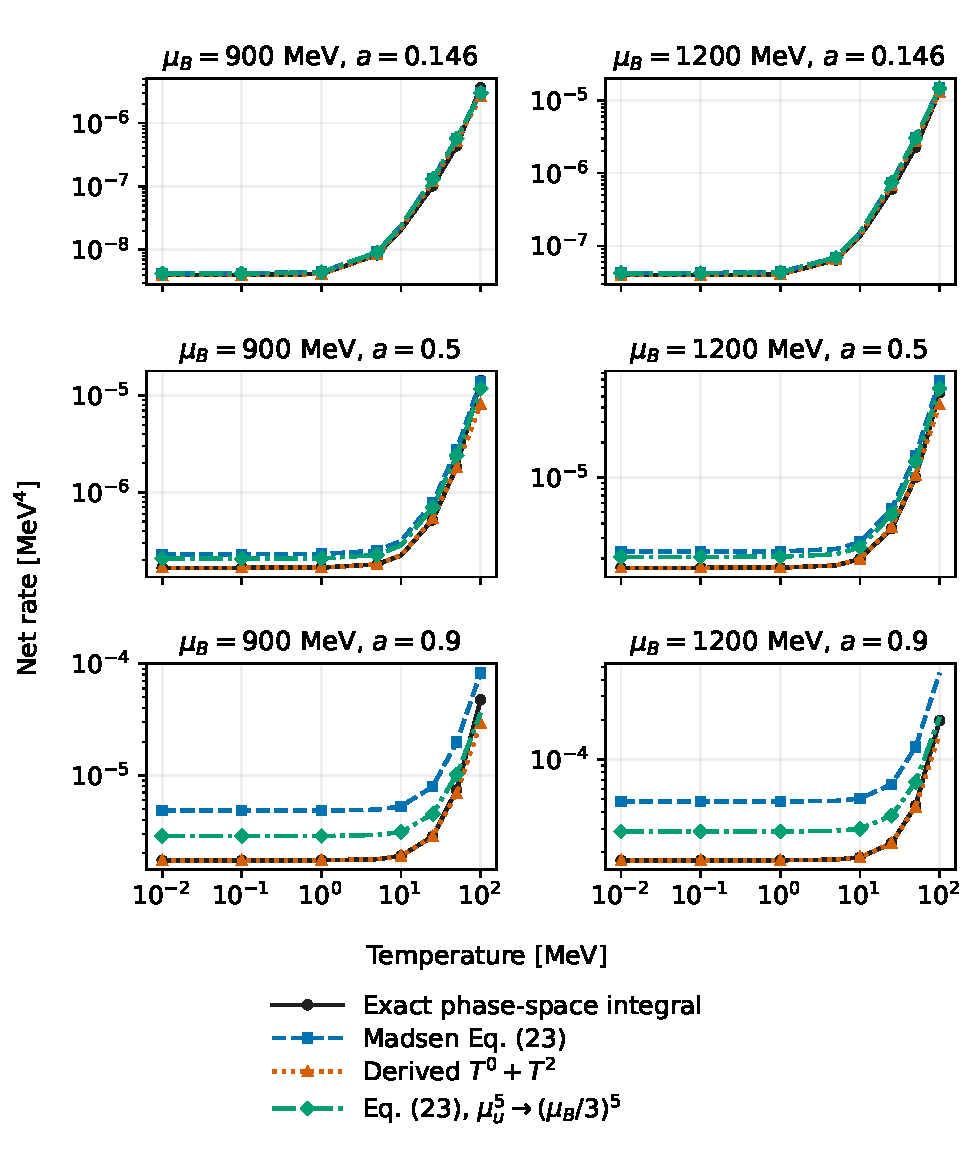
\includegraphics[width=\textwidth]{results/exact-rates.pdf}
 \caption{Absolute net quark-channel rates for the four local-rate models, at \(\mu_B=900\) and \(1200\,\MeV\) and fixed compositions \(a=0.146,0.5,0.9\).
 Black is the exact phase-space integral, blue is Madsen's Eq.~(23), orange is the derived \(T^0+T^2\) rate, and green is Eq.~(23) with \(\mu_u^5\to(\mu_B/3)^5\).
 All values are in natural units.
 The black and orange curves nearly coincide at low temperature; their separation at higher temperature measures the truncation error.}
 \label{fig:exact-rates}
\end{figure}
\begin{figure}[p]
 \centering
 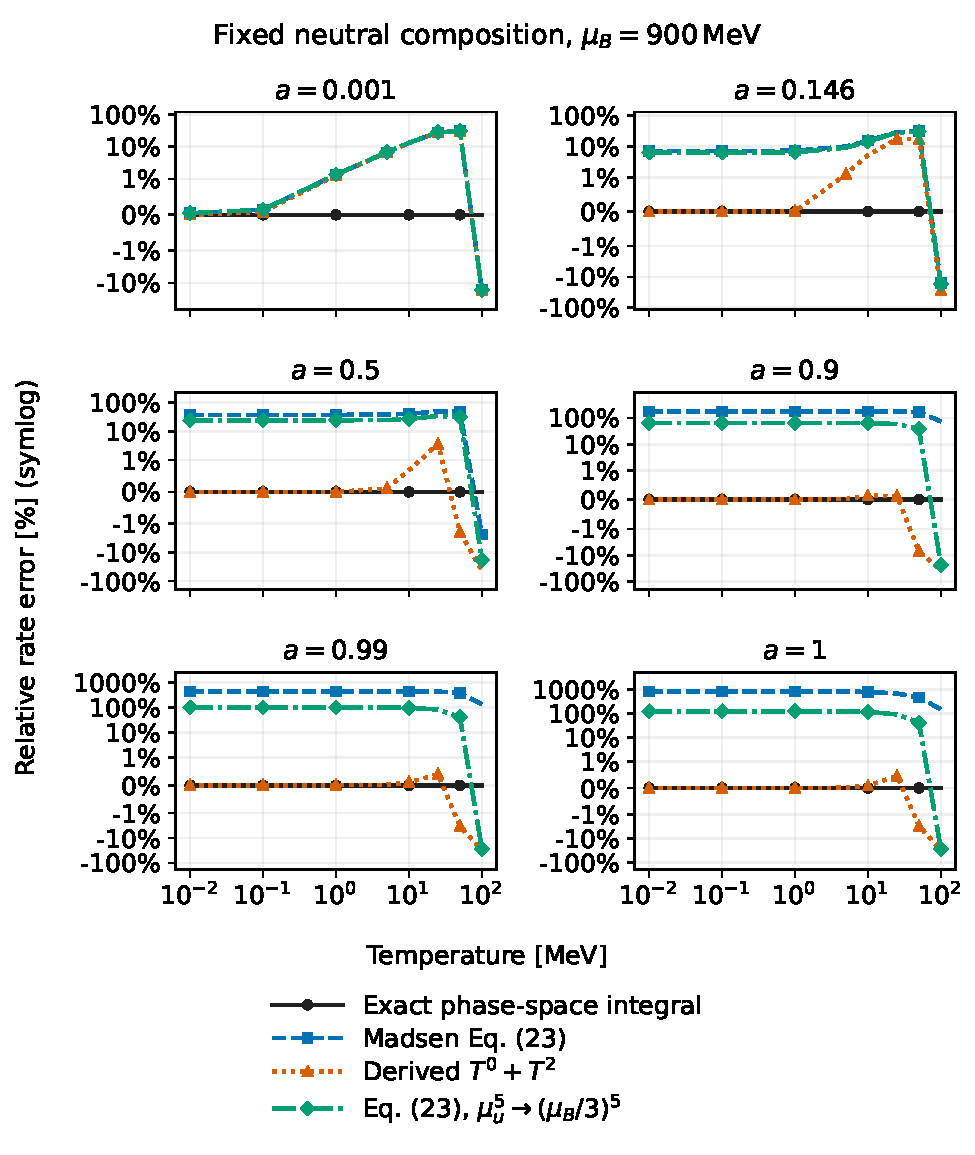
\includegraphics[width=\textwidth]{results/approximation-errors-muB-900.pdf}
 \caption{Relative local-rate errors, \(100(\Gamma_K/\Gamma_{K,\mathrm{exact}}-1)\), at fixed neutral composition and \(\mu_B=900\,\MeV\).
 The exact phase-space integral (black) defines zero error; blue is Madsen's Eq.~(23), orange is the derived \(T^0+T^2\) rate, and green is Eq.~(23) with \(\mu_u^5\to(\mu_B/3)^5\).
 The vertical scale is linear within \(1\%\) of zero and logarithmic outside that range.
 Lines connect the eight tested temperatures; they are not additional validation points.}
 \label{fig:errors-900}
\end{figure}
\begin{figure}[p]
 \centering
 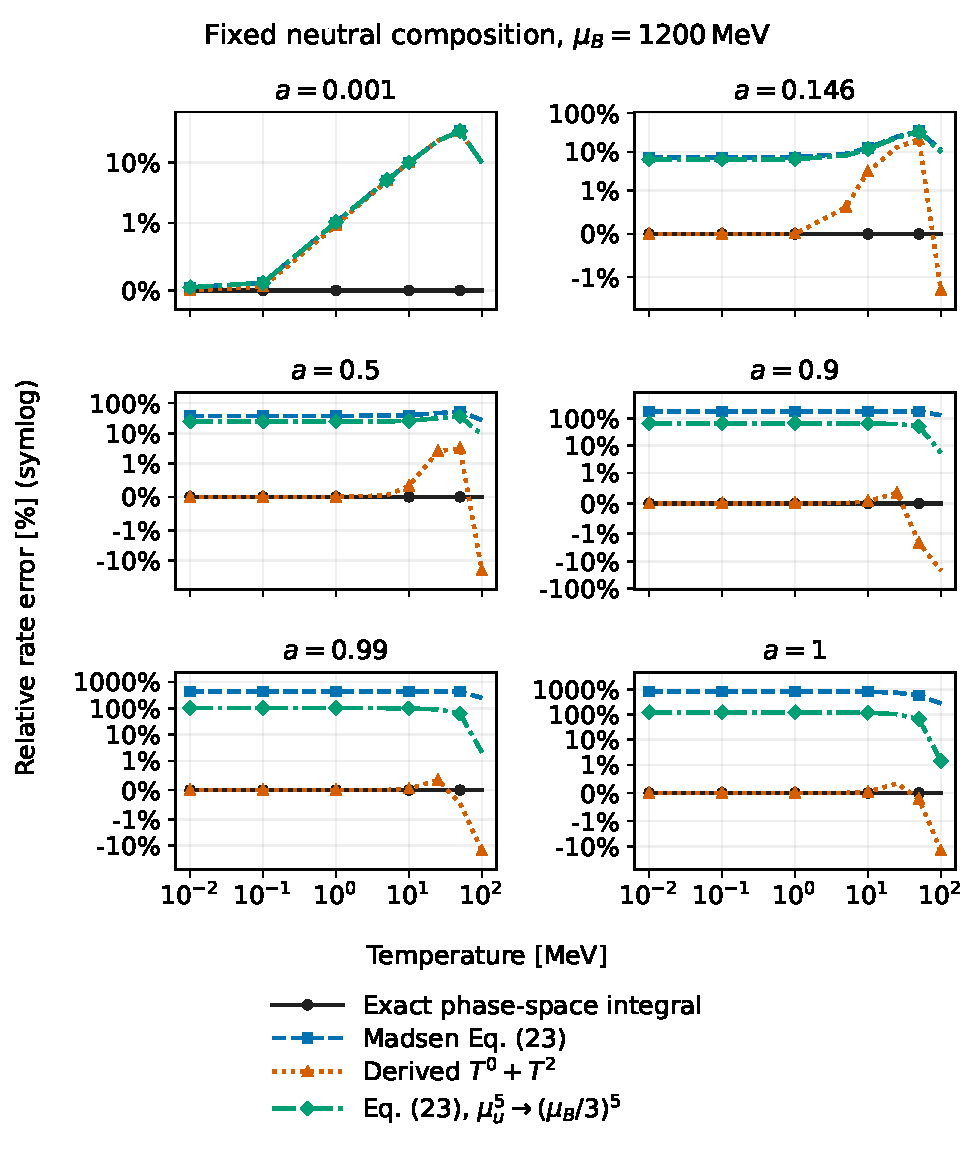
\includegraphics[width=\textwidth]{results/approximation-errors-muB-1200.pdf}
 \caption{The same comparison as \cref{fig:errors-900}, at \(\mu_B=1200\,\MeV\).
 Raising the chemical-potential scale reduces \(T/\mu_B\) at fixed dimensional temperature; the resulting error need not decrease monotonically outside the low-temperature regime.}
 \label{fig:errors-1200}
\end{figure}
These figures compare local reaction rates; the following integral comparison estimates their effect on a speed without solving a front.

\clearpage
\subsection{Isothermal speed sensitivity at fixed background}
The conversion-front speed depends on the rate integrated over composition, rather than on the rate at the interface alone.
To isolate this dependence, hold the diffusion and baryon-density prefactors constant and identical between models, together with the interface and profile-shape factors in the speed estimate.
Writing \(\Gamma_{K,\rm exact}\) for the exact phase-space rate, the ratio to its speed estimate is then
\begin{equation}
 \frac{u_{\rm est}(0^-)}{u_{{\rm exact},\rm est}(0^-)}
 =\left[
 \frac{\displaystyle\int_0^{a(0^+)}\Gamma_K\,\dd a}
 {\displaystyle\int_0^{a(0^+)}\Gamma_{K,\rm exact}\,\dd a}
 \right]^{1/2}.
 \label{eq:speed-sensitivity}
\end{equation}
Each integrand is evaluated on the neutral EOS at fixed \(\mu_B=1200\,\MeV\) and fixed temperature, with the chemical potentials recalculated at each composition.
This path is a rate comparison, not a reconstructed constant-pressure front.
The four choices of \(\Gamma_K\) are the rate models of the local-rate figures.
Figure~\ref{fig:speed-sensitivity} shows the cold-rate limit and \(T=20,50,100\,\MeV\), with the exact estimate equal to one by definition.
At \(T=0\), the exact integral and the derived \(T^0+T^2\) rate give the same result, so their curves coincide.
At \(a(0^+)=1\), the \((\mu_B/3)^5\) variant gives \(1.29\), \(1.27\), \(1.22\), and \(1.03\) at \(T=0,20,50,100\,\MeV\), compared with \(1.77\), \(1.75\), \(1.68\), and \(1.43\) for Eq.~(23).
The cold panel is a limiting ratio of rate integrals, not a claim that the diffusion coefficient or an absolute isothermal speed remains finite at zero temperature.
None of these panels is a re-solved boundary-value problem; changes in the hydrodynamic trajectory and the diffusion-profile shape are not included.
The point \(a(0^+)=1\) is only the endpoint of this rate-integral comparison, not a finite-speed front solution.
\par
Increasing the outer Gauss--Legendre order from 12 to 16 and the phase-space order from 24 to 32, while extending the thermal tail from \(48T\) to \(64T\), changes the integrated exact rate by at most \(5.57\times10^{-9}\) relative across the sampled compositions.
The corresponding maximum changes for Eq.~(23) and the derived \(T^0+T^2\) expression are \(2.09\times10^{-8}\) and \(5.58\times10^{-9}\), respectively.
Independent checks at \(T=50,100\,\mathrm{MeV}\) and \(a(0^+)=0.146,0.5,0.9\) increase only the outer order from 16 to 24, only the phase-space order from 32 to 40, or only the tail from \(64T\) to \(80T\).
Including a comparison of the benchmark and plotted composition partitions, the largest relative change of any speed ratio is \(2.35\times10^{-12}\), below the \(10^{-3}\) acceptance tolerance.

\begin{table}[htbp]
\centering
\caption{Percentage change of the rate-integral speed estimate relative to the exact phase-space result, whose change is identically zero, at \(\mu_B=1200\,\mathrm{MeV}\).}
\label{tab:speed-sensitivity}
\begin{tabular}{rr rr}
\toprule
\(T\,[\mathrm{MeV}]\) & \(a(0^+)\) & Eq.~(23) & Derived \(T^0+T^2\) \\
\midrule
0 & 0.146 & \(+2.78\%\) & \(0.00\%\) \\
0 & 0.5 & \(+12.86\%\) & \(0.00\%\) \\
0 & 0.9 & \(+42.41\%\) & \(0.00\%\) \\
\addlinespace
20 & 0.146 & \(+9.51\%\) & \(+6.09\%\) \\
20 & 0.5 & \(+15.20\%\) & \(+2.00\%\) \\
20 & 0.9 & \(+40.90\%\) & \(+0.51\%\) \\
\addlinespace
50 & 0.146 & \(+15.61\%\) & \(+11.70\%\) \\
50 & 0.5 & \(+19.61\%\) & \(+4.95\%\) \\
50 & 0.9 & \(+39.35\%\) & \(+0.51\%\) \\
\addlinespace
100 & 0.146 & \(+5.14\%\) & \(+0.81\%\) \\
100 & 0.5 & \(+8.76\%\) & \(-7.06\%\) \\
100 & 0.9 & \(+25.89\%\) & \(-11.58\%\) \\
\bottomrule
\end{tabular}
\end{table}

At \(T=20\,\mathrm{MeV}\) and \(a(0^+)=0.146\), Eq.~(23) and the derived \(T^0+T^2\) rate give speed-estimate changes relative to the exact result of \(+9.51\%\) and \(+6.09\%\); at \(a(0^+)=0.9\), the changes are \(+40.90\%\) and \(+0.51\%\), respectively.
At \(T=50\,\mathrm{MeV}\) and \(a(0^+)=0.146\), Eq.~(23) and the derived \(T^0+T^2\) rate give speed-estimate changes relative to the exact result of \(+15.61\%\) and \(+11.70\%\); at \(a(0^+)=0.9\), the changes are \(+39.35\%\) and \(+0.51\%\), respectively.
At \(T=100\,\mathrm{MeV}\) and \(a(0^+)=0.146\), Eq.~(23) and the derived \(T^0+T^2\) rate give speed-estimate changes relative to the exact result of \(+5.14\%\) and \(+0.81\%\); at \(a(0^+)=0.9\), the changes are \(+25.89\%\) and \(-11.58\%\), respectively.
The hot points test the finite-temperature rate prescriptions within the same four-quark channel; agreement there does not establish a uniformly valid low-temperature expansion or a re-solved front speed.


\begin{figure}[!htbp]
 \centering
 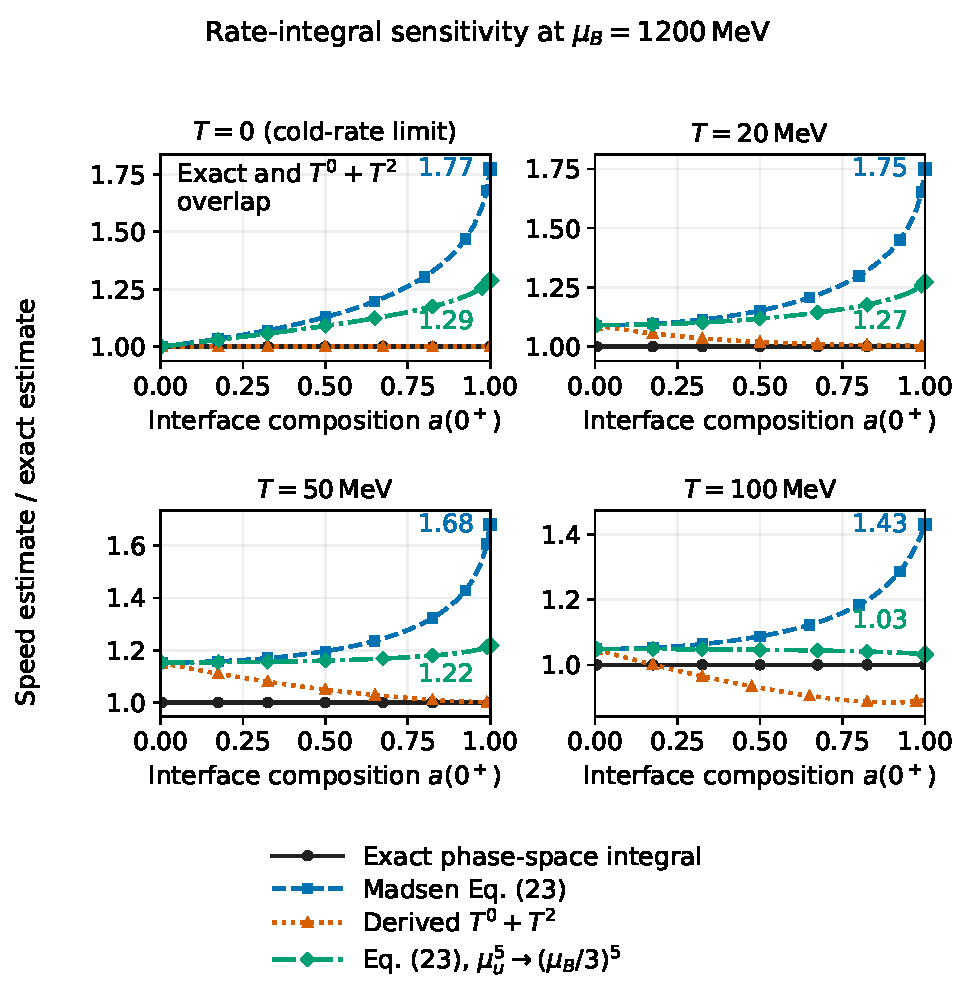
\includegraphics[width=\textwidth]{results/speed-sensitivity.pdf}
 \caption{Isothermal rate-integral speed estimates from \cref{eq:speed-sensitivity}, relative to the exact phase-space estimate, at \(\mu_B=1200\,\MeV\) and \(T=0,20,50,100\,\MeV\).
 The four rate models use the same colors and line styles as the local-rate figures; blue and green labels give the Eq.~(23) and \((\mu_B/3)^5\) ratios at \(a(0^+)=1\).
 The exact phase-space and \(T^0+T^2\) curves coincide in the cold panel, which is explicitly a limiting rate-integral ratio.
 Only the reaction rate changes between models; these are sensitivity estimates, not numerically solved front velocities.}
 \label{fig:speed-sensitivity}
\end{figure}
\clearpage
\subsection{Adiabatic speed sensitivity along the conserved EOS trajectory}
\label{sec:adiabatic-sensitivity}
For an adiabatic conversion layer, the temperature-dependent diffusion coefficient must remain inside the rate integral.
We reconstruct the thermodynamic trajectory from upstream conditions, using the slow-front conservation laws and imposing a cold quark interface, \(T(0^+)=0\).
The inputs are \(T(0^-)\) and \(n_B(0^-)\); neither a quark-side chemical potential nor the equilibrated downstream temperature is prescribed.
The upstream phase is QMC-RMF3 pure neutron matter~\cite{Alford:2022bpp,Alford:2023rgp}, with \(n_0=0.16\,\mathrm{fm}^{-3}\), and the bag calibration is \(U_{\rm bag}^{1/4}=189.1566\,\MeV\).
We scan \(1\le n_B(0^-)/n_0\le10\) at \(T(0^-)=0,0.1,5,20,50,100\,\MeV\), refine the boundaries of admissible intervals, and solve for the requested interface compositions within those intervals.
Each slice starts from a 73-point density grid, followed by root refinement and composition-targeted sampling; these reported intervals are numerical scan results rather than a proof excluding arbitrarily narrow disconnected branches.

\paragraph{Conserved trajectory.}
The slow-front constraints are
\begin{equation}
 P(a)=P(0^-),\qquad
 \frac{h(a)}{n_B(a)}=\frac{h(0^-)}{n_B(0^-)}.
 \label{eq:adiabatic-conservation}
\end{equation}
For the massless bag EOS including thermal gluons,
\begin{align}
 P+U_{\rm bag}
 &=\sum_{f=u,d,s}\left(\frac{\mu_f^4}{4\pi^2}+\frac{\mu_f^2T^2}{2}\right)
   +\frac{19\pi^2T^4}{36},\label{eq:adiabatic-pressure}\\
 h&=4(P+U_{\rm bag}),\qquad
 n_B=\frac{4[P(0^-)+U_{\rm bag}]}{h(0^-)/n_B(0^-)}.
 \label{eq:adiabatic-density}
\end{align}
Thus constant baryon density on the quark trajectory follows from conservation and this EOS; it is not an additional frozen-background approximation.
The neutral densities are those of \cref{eq:density}.
The cold interface is found from
\begin{equation}
 P(0^-)+U_{\rm bag}
 =\frac{(\pi^2n_B)^{4/3}}{4\pi^2}
 \left\{1+[1+a(0^+)]^{4/3}+[1-a(0^+)]^{4/3}\right\}.
 \label{eq:adiabatic-cold-interface}
\end{equation}
We retain only \(0<a(0^+)<1\).
For each retained state, solving \cref{eq:density,eq:adiabatic-pressure} at decreasing composition gives \(T(a)\) and all three flavor potentials, ending at \(a(\infty)=0\) and \(\mu_K(\infty)=0\).
The resulting \(T(\infty)\) is an output, and \(\mu_B(a)\) varies along the path.
The neutron-matter roots are required to satisfy the existing physical-branch and residual checks and to agree from at least two seeds.
Supplemental initial seeds recover failed roots without changing these criteria or the production EOS files.

\paragraph{Diffusion-weighted comparison.}
At the same local EOS states for every rate prescription, define
\begin{equation}
 I_{2,\mathrm{model}}=\frac1{n_B}\int_0^{a(0^+)}
 D_K(a)\,\Gamma_{K,\mathrm{model}}(a)\,\dd a,
 \qquad
 \frac{u_{\mathrm{model,est}}(0^-)}{u_{\mathrm{exact,est}}(0^-)}
 =\left(\frac{I_{2,\mathrm{model}}}{I_{2,\mathrm{exact}}}\right)^{1/2}.
 \label{eq:adiabatic-speed-ratio}
\end{equation}
Interface factors and the profile-shape parameter \(\xi\) are identical between models.
We use both terms of the existing diffusion prescription~\cite{Heiselberg:1993cr},
\begin{equation}
 D_K^{-1}=\frac{24\alpha_s^2}{\pi}
 \left[h_D\frac{T^{5/3}}{q_D^{2/3}}+\frac{\pi^3T^2}{12q_D}\right],
 \quad q_D=\sqrt{\frac{6\alpha_s}{\pi}}\frac{\mu_B}{3},
 \quad \alpha_s=0.3,\quad h_D=1.81317,
 \label{eq:adiabatic-diffusion}
\end{equation}
with the local temperature and baryon chemical potential.
The strong coupling enters this transport prescription; the rate still uses the tree-level four-quark channel specified in \cref{sec:conventions}.

\paragraph{The cold endpoint.}
For a fixed interior interface composition, the cold constant-density pressure derivatives give
\begin{equation}
 \left.\frac{\partial P}{\partial a}\right|_{n_B,T=0}
 =\frac{n_B(\mu_d-\mu_s)}3,
 \qquad
 \lim_{T\to0^+}\frac1T\left.\frac{\partial P}{\partial T}\right|_{n_B,a}
 =\frac{\mu_u^2+\mu_d^2+\mu_s^2}{3}.
 \label{eq:adiabatic-cold-derivatives}
\end{equation}
Consequently \(|\dd a/\dd T|\propto T\), whereas \(D_K\propto T^{-5/3}\), so \(D_K\Gamma_K|\dd a/\dd T|\propto T^{-2/3}\) is integrable.
The dimensionless integration coordinate \(z=[T/T(\infty)]^{1/3}\) removes this singularity and runs from the cold interface to equilibrium.
Its EOS Jacobian is obtained by implicit differentiation of \cref{eq:adiabatic-pressure} at fixed density:
\begin{equation}
 \left|\frac{\dd a}{\dd z}\right|
 =\frac{(\partial P/\partial T)_{n_B,a}}{(\partial P/\partial a)_{n_B,T}}
 \,3T(\infty)z^2.
 \label{eq:adiabatic-jacobian}
\end{equation}
The finite cold value of the transformed integrand is
\begin{equation}
 \lim_{z\to0^+}\frac{D_K\Gamma_K}{n_B}\left|\frac{\dd a}{\dd z}\right|
 =\frac{\pi q_D(0^+)^{2/3}\Gamma_K(0^+)T(\infty)^{1/3}
         \sum_f\mu_f(0^+)^2}
 {8\alpha_s^2h_D n_B^2[\mu_d(0^+)-\mu_s(0^+)]}.
 \label{eq:adiabatic-cold-integrand}
\end{equation}
No temperature floor is inserted.
This improper integral defines a formal speed sensitivity with the stated transport law; its finiteness does not establish the validity of local diffusion arbitrarily close to a zero-temperature interface.

\paragraph{Results and diffusion weighting.}
With \(T(0^+)=0\), the interface composition is an output rather than an input.
Eliminating \(n_B\) between \cref{eq:adiabatic-density,eq:adiabatic-cold-interface} gives
\begin{equation}
 1+[1+a(0^+)]^{4/3}+[1-a(0^+)]^{4/3}
 =\left[\frac{(h/n_B)^4}{4\pi^2(P+U_{\rm bag})}\right]^{1/3}_{0^-},
 \label{eq:adiabatic-composition-map}
\end{equation}
so each upstream state \((n_B(0^-),T(0^-))\) fixes one composition, with \(a(0^+)=0\) and \(a(0^+)=1\) at right-hand values \(3\) and \(1+2^{4/3}\).
At fixed \(a(0^+)\), this massless cold-interface problem has a useful scaling property.
All temperatures and chemical potentials scale as \(n_B^{1/3}\), the weak rate as \(n_B^{8/3}\), diffusion as \(n_B^{-1/3}\), and hence \(I_2\) as \(n_B^{4/3}\).
The two-term diffusion law preserves this scaling at fixed \(\alpha_s\).
Therefore the ratios in \cref{eq:adiabatic-speed-ratio} depend on the upstream state only through \(a(0^+)\), and lines of constant ratio in the upstream plane are lines of constant \(a(0^+)\).
Figure~\ref{fig:adiabatic-speed} shows these lines in the \((n_B(0^-),T(0^-))\) plane used for the front-speed contours.
The right side of \cref{eq:adiabatic-composition-map} is evaluated with the same QMC-RMF3 validator on a uniform grid of 49 temperatures from \(0\) to \(120\,\MeV\) and 101 densities from \(n_0\) to \(6n_0\), with no EOS failures.
The grid encloses both boundaries; the \(a(0^+)=1\) boundary reaches \(n_B(0^-)=n_0\) at \(T(0^-)=112.28\,\MeV\).
Each contour level is converted to a composition with the composition-resolved quadrature of this section, whose ratio curves appear in the left panel of Figure~\ref{fig:adiabatic-diffusion}.
At the 128 precisely solved upstream states inside this grid, the linearly interpolated composition differs from the solved one by at most \(2.6\times10^{-3}\).
Only interior compositions are integrated; the largest composition in the quadrature is \(0.995\), and neither endpoint is asserted to be a finite-speed solution.
For \(T(0^-)\leq50\,\MeV\), the scanned densities span the full interior composition interval.
At \(T(0^-)=100\,\MeV\), the density interval is \([1,3.380011)\,n_0\) and the attainable composition interval is \([0.879368,1)\).
Here the composition initially decreases with density, reaches its minimum at \(n_B(0^-)/n_0=1.444184\), and then increases.
Both density roots are saved for the sampled compositions \(0.88,0.885,0.89\); they produce the same speed ratio by the scaling above.
The complete selection contains 153 upstream states at 45 distinct interface compositions, with no unresolved EOS queries.
\par
\begin{table}[tbp]
\centering
\caption{Adiabatic cold-interface benchmarks on the conserved EOS trajectory.
The last two columns give percentage changes of the speed estimate relative to the exact phase-space reference.}
\label{tab:adiabatic-speed}
\begin{tabular}{rrrrrr}
\toprule
\(T(0^-)\) & \(a(0^+)\) & \(n_B(0^-)/n_0\) & \(T(\infty)\) & Eq.~(23) & \(T^0+T^2\)\\
{[MeV]} & & & {[MeV]} & {[\%]} & {[\%]}\\
\midrule
0 & 0.146 & 3.04060 & 8.726 & +3.70 & +0.35 \\
0 & 0.5 & 3.48993 & 31.097 & +16.66 & +0.81 \\
0 & 0.9 & 4.75287 & 63.297 & +56.11 & +0.46 \\
0.1 & 0.146 & 3.04060 & 8.726 & +3.70 & +0.35 \\
0.1 & 0.5 & 3.48993 & 31.097 & +16.66 & +0.81 \\
0.1 & 0.9 & 4.75287 & 63.297 & +56.11 & +0.46 \\
5 & 0.146 & 3.03437 & 8.723 & +3.70 & +0.35 \\
5 & 0.5 & 3.48461 & 31.086 & +16.66 & +0.81 \\
5 & 0.9 & 4.74894 & 63.280 & +56.11 & +0.46 \\
20 & 0.146 & 2.93742 & 8.671 & +3.70 & +0.35 \\
20 & 0.5 & 3.40278 & 30.911 & +16.66 & +0.81 \\
20 & 0.9 & 4.68940 & 63.009 & +56.11 & +0.46 \\
50 & 0.146 & 2.22564 & 8.352 & +3.70 & +0.35 \\
50 & 0.5 & 2.85750 & 29.844 & +16.66 & +0.81 \\
50 & 0.9 & 4.33343 & 61.411 & +56.11 & +0.46 \\
100 & 0.146 & \multicolumn{4}{c}{unavailable in density search range}\\
100 & 0.5 & \multicolumn{4}{c}{unavailable in density search range}\\
100 & 0.9 & 2.08661 & 52.968 & +56.11 & +0.46 \\
\bottomrule
\end{tabular}
\end{table}
The unavailable benchmark compositions at \(T(0^-)=100\,\mathrm{MeV}\) are \(0.146\), \(0.5\).
\begin{table}[tbp]
\centering
\caption{Admissible upstream density intervals in the search range \(1\le n_B(0^-)/n_0\le10\).
Boundary compositions \(0\) and \(1\) are limiting states, excluded from the rate-integral calculation.}
\label{tab:adiabatic-intervals}
\begin{tabular}{rccc}
\toprule
\(T(0^-)\) [MeV] & \(n_B(0^-)/n_0\) interval & limiting \(a(0^+)\) range & status\\
\midrule
0 & (3.000000, 5.297929) & (0.0000, 1.0000) & admissible \\
0.1 & (2.999998, 5.297932) & (0.0000, 1.0000) & admissible \\
5 & (2.993658, 5.294344) & (0.0000, 1.0000) & admissible \\
20 & (2.894983, 5.240216) & (0.0000, 1.0000) & admissible \\
50 & (2.160893, 4.923040) & (0.0000, 1.0000) & admissible \\
100 & [1.000000, 3.380011) & [0.8794, 1.0000) & admissible \\
\bottomrule
\end{tabular}
\end{table}
At \(a(0^+)=0.146,0.5,0.9\), Eq.~(23) gives speed-estimate changes of \(+3.70\%\), \(+16.66\%\), \(+56.11\%\), respectively.
At the same compositions the derived \(T^0+T^2\) prescription changes the estimate by \(+0.35\%\), \(+0.81\%\), \(+0.46\%\).
For \(a(0^+)=0.9\), replacing local diffusion by a common constant on the same thermodynamic trajectory changes the Eq.~(23) ratio from \(1.56107\) to \(1.32678\).


Figure~\ref{fig:adiabatic-diagnostics} shows the temperature, diffusion coefficient, local rate error, and cumulative contribution for a representative trajectory, including the \((\mu_B/3)^5\) variant of Eq.~(23).
On this trajectory the variant gives a speed ratio of \(1.252\), compared with \(1.561\) for Eq.~(23).
The large diffusion coefficient gives additional weight to the cold, unequilibrated part of the path, where the mismatch between the exact cold phase space and Eq.~(23) is substantial.
Figure~\ref{fig:adiabatic-diffusion} repeats the comparison after replacing diffusion by one common constant on each of the same trajectories.
This diagnostic isolates diffusion weighting while keeping the thermodynamic path and all local rates unchanged.
Agreement of the integrated \(T^0+T^2\) prescription with the exact reference is an observed weighted result, not a claim of uniform accuracy of the temperature expansion near equilibrium or at high temperature.
\paragraph{Verification.}
Across 11,016 saved dimensional trajectory samples, the maximum relative pressure and enthalpy-per-baryon residuals are \(6.58\times10^{-13}\), while the neutrality and baryon-density residuals are below \(4\times10^{-15}\).
Every reconstructed trajectory has \(T(0^+)=0\) and \(\mu_K(\infty)=0\); the maximum mismatch between target and solved interface composition is \(8.98\times10^{-12}\).
% Generated by adiabatic_verify.py; do not edit by hand.
Numerical verification covers 45 distinct interface compositions and 143 quadrature records.
Outer-order refinement covers every composition; phase-order and tail checks cover four representative compositions.
The cold-state sweep evaluates 3025 states, with 0 failures and maximum relative pressure and density residuals \(6.66\times10^{-16}\) and \(6.66\times10^{-16}\), respectively.
An independently implemented 40-digit EOS and composition-coordinate integral check the temperature-coordinate Jacobian; the rate and diffusion routines are shared.
\par
\begin{table}[htbp]
\centering
\small
\begin{tabular}{lrr}
\hline
Check & Integral change & Speed-ratio change \\
\hline
Independent coordinate & \(4.19\times10^{-6}\) & \(2.10\times10^{-6}\) \\
EOS iterations 64 to 100 & \(0\) & \(0\) \\
Outer order 12 to 18 & \(9.44\times10^{-6}\) & \(4.72\times10^{-6}\) \\
Phase order 16 to 28 & \(2.22\times10^{-16}\) & \(2.22\times10^{-16}\) \\
Tail 48 to 64 & \(4.44\times10^{-16}\) & \(2.22\times10^{-16}\) \\
Cutoff \(1.00\times10^{-3}\), uncorrected & \(1.30\times10^{-1}\) & \(9.12\times10^{-3}\) \\
Cutoff \(1.00\times10^{-3}\), cold tail added & \(5.39\times10^{-3}\) & \(3.33\times10^{-4}\) \\
Cutoff \(1.00\times10^{-5}\), uncorrected & \(2.88\times10^{-2}\) & \(1.84\times10^{-3}\) \\
Cutoff \(1.00\times10^{-5}\), cold tail added & \(2.61\times10^{-4}\) & \(1.62\times10^{-5}\) \\
Cutoff \(1.00\times10^{-7}\), uncorrected & \(6.26\times10^{-3}\) & \(3.90\times10^{-4}\) \\
Cutoff \(1.00\times10^{-7}\), cold tail added & \(1.22\times10^{-5}\) & \(6.07\times10^{-6}\) \\
\hline
\end{tabular}
\caption{Observed relative numerical changes for the cold-interface adiabatic sensitivity calculation, taking the maximum absolute value over the tested compositions and rate models.
Cutoffs are specified by \(T_{\rm cut}/T(\infty)\); uncorrected rows intentionally omit the cold contribution and are not acceptance checks.
Every independent, refined, and corrected speed ratio agrees within the required relative tolerance \(10^{-3}\).}
\label{tab:adiabatic-verification}
\end{table}
\par

\par
These are semi-analytical sensitivities of a shared-trajectory, fixed-profile speed estimate.
No spatial boundary-value problem, absolute velocity, or rate-dependent change of \(\xi\) has been calculated.

\begin{figure}[p]
 \centering
 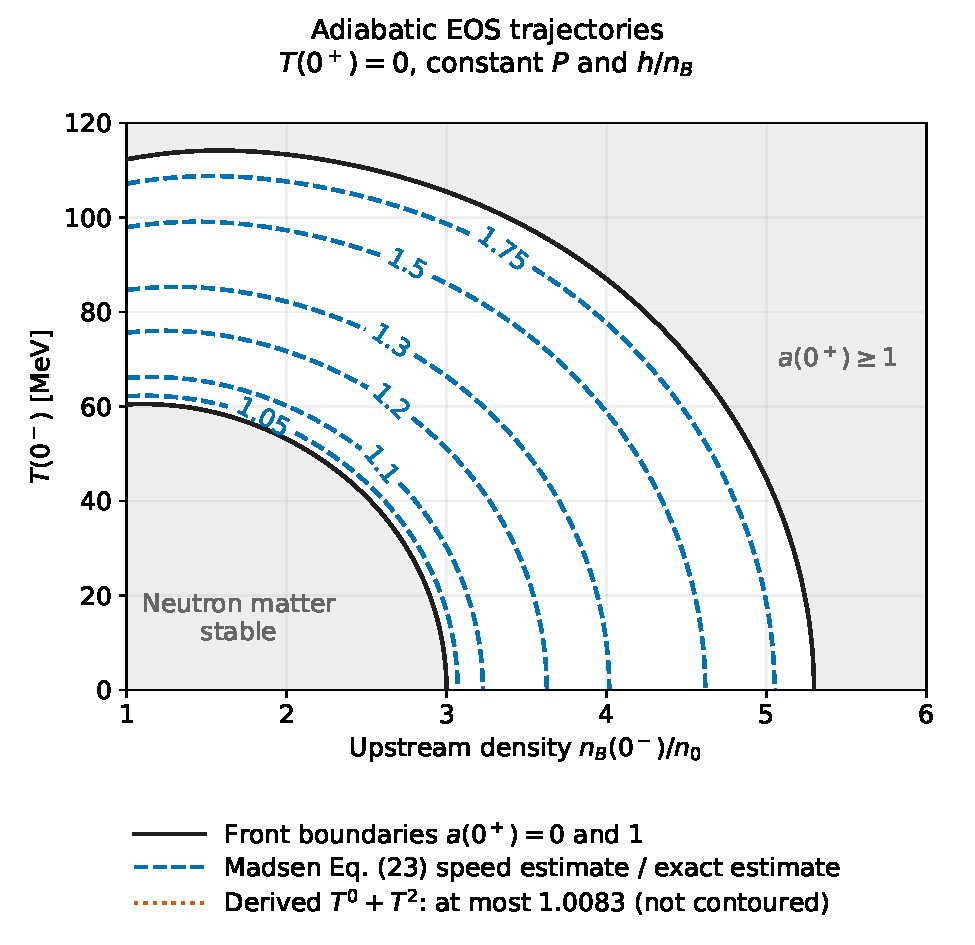
\includegraphics[width=\textwidth]{results/adiabatic-speed-map.pdf}
 \caption{Adiabatic rate-integral speed estimates over upstream QMC-RMF3 neutron-matter states, with \(T(0^+)=0\) and the conserved EOS trajectory.
 Blue dashed contours give the Eq.~(23) estimate divided by the exact phase-space estimate, with local diffusion inside \(I_2\); by massless scaling each contour is a line of constant \(a(0^+)\).
 Black lines are the boundaries \(a(0^+)=0\) and \(a(0^+)=1\); the shaded regions have no cold-interface front.
 The derived \(T^0+T^2\) ratio is at most \(1.0083\) at every computed composition and is not contoured.
 Contours are interpolated from the upstream grid described in the text, whose density range starts at \(n_0\).}
 \label{fig:adiabatic-speed}
\end{figure}
\begin{figure}[p]
 \centering
 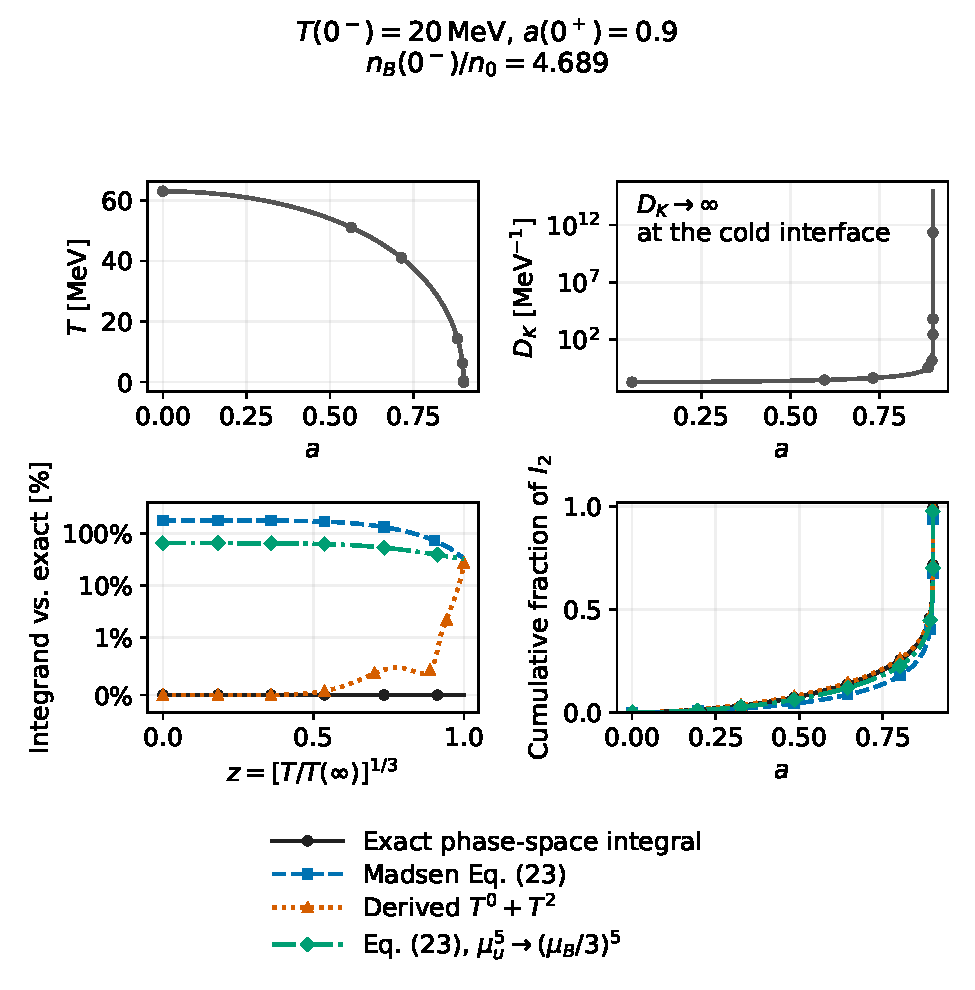
\includegraphics[width=\textwidth]{results/adiabatic-trajectory-diagnostics.pdf}
 \caption{A representative conserved trajectory at \(T(0^-)=20\,\MeV\) and \(a(0^+)=0.9\).
 The upper panels show temperature and local diffusion; diffusion diverges at the cold interface.
 The lower left panel shows each weighted integrand \((D_K\Gamma_K/n_B)|\dd a/\dd z|\) relative to the exact one, in percent on a linear scale within \(1\%\) of zero and logarithmic outside it.
 Because \(D_K\) and the Jacobian are common to all models, this is the local rate error along the path; it is finite at the cold limit \(z=0\).
 Green is Eq.~(23) with \(\mu_u^5\to(\mu_B/3)^5\).
 The lower right panel shows the contribution accumulated from equilibrium to the indicated composition, normalized separately by each model's total \(I_2\).
 Curves connect quadrature samples.}
 \label{fig:adiabatic-diagnostics}
\end{figure}
\begin{figure}[p]
 \centering
 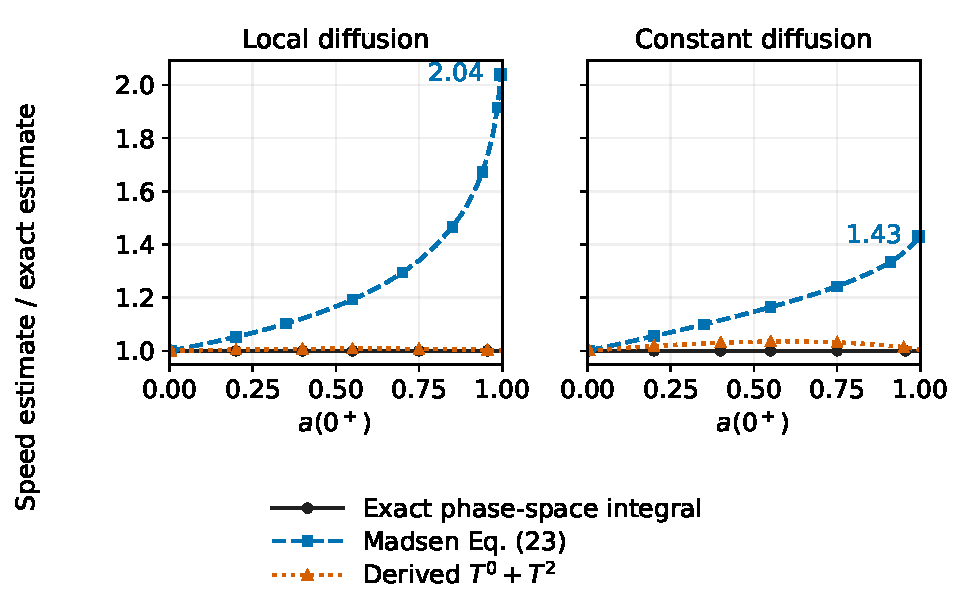
\includegraphics[width=\textwidth]{results/adiabatic-diffusion-weighting.pdf}
 \caption{Local-diffusion and constant-diffusion comparisons on identical adiabatic EOS trajectories.
 In the right panel, a common constant diffusion coefficient cancels from the ratio.
 Both panels retain the temperature rise and varying flavor chemical potentials.
 All three rate prescriptions follow the same color and line conventions as Figure~\ref{fig:speed-sensitivity}.}
 \label{fig:adiabatic-diffusion}
\end{figure}



\clearpage
\section{Use of the result}
The rate derived here is exact at zero temperature within the stated massless, tree-level quark-channel model, and its thermal coefficient retains the physical composition dependence.
The low-temperature formula must be used with its branch and degeneracy conditions, especially near a vanishing strange Fermi surface or simultaneous small temperature and imbalance.
For warmer states, \cref{eq:exact-2d} supplies a reference without a temperature expansion.
Neutral massless matter has only two dimensionless state variables, which may be chosen as \(a\) and \(T/\mu_B\); the rate scales as \(G_F^2\sin^2\theta_C\cos^2\theta_C\mu_B^8\).
A later production implementation can therefore tabulate a dimensionless rate and match it to the cold expression, without evaluating phase space during every front-solver call.
No production solver or combustion-manuscript formula has been replaced as part of this derivation.

\appendix
\section{Spin traces and angular normalization}
\label{app:normalization}
With \(L=1-\gamma^5\), the spin sum from \cref{eq:interaction} is proportional to
\begin{align}
 &\operatorname{tr}[\slashed p_2\gamma^\alpha L\slashed p_d\gamma^\beta L]
 \operatorname{tr}[\slashed p_s\gamma_\alpha L\slashed p_1\gamma_\beta L]
 =256(p_1\cdot p_d)(p_2\cdot p_s).
 \label{eq:spin-trace}
\end{align}
Multiplication by the squared coupling \(G_F^2\sin^2\theta_C\cos^2\theta_C/2\) gives the spin-summed factor quoted in the main text.
The file \texttt{spin-trace.wl} verifies \cref{eq:spin-trace} with explicit Dirac matrices and the \(+---\) metric.
For the angular convolution, align \(\bm k\) with the polar axis and integrate the second direction using the three-dimensional delta function.
The remaining delta function is \(\delta(|\bm k-\bm p_1|-E_d)/E_d^2\), whose polar-angle Jacobian is \(E_d/(kE_1)\).
The azimuthal integral gives \(2\pi\), and requiring a polar cosine between \(-1\) and \(1\) gives the triangle inequalities in \cref{eq:pair-angle}.
The normalization after the four radial measures and this angular integration is explicitly
\begin{equation}
 \frac{18\times64}{4}\,
 \frac{(2\pi)^4}{(2\pi)^{12}2^4}\,16\pi^3
 =\frac{9}{8\pi^5},
 \label{eq:normalization-arithmetic}
\end{equation}
where the first factor \(1/4\) comes from the two invariant dot products, and the factors of the four energies cancel.

\section{Polynomial cold integrations}
\label{app:cold-algebra}
An antiderivative of the angular kernel with respect to pair energy is
\begin{equation}
 \int\mathcal K(E,m)\dd E
 =\frac{32}{9}E^3m^3-8E^2m^4+\frac{32}{5}Em^5.
 \label{eq:energy-primitive}
\end{equation}
After inserting the energy bounds in \cref{eq:cold-triple} and integrating over \(y\), the three regions described in \cref{sec:cold} give the following one-dimensional integrands:
\begin{align}
 F_1(x)={}&\frac{8x^3}{45}(x+\mu_d-\mu_s-\mu_u)^2
 \Big[15\mu_d^2+10\mu_d(\mu_s+\mu_u)\notag\\
 &\hspace{30mm}+5(\mu_s+\mu_u)^2-5(\mu_s+\mu_u)x+3x^2\Big],
 \label{eq:region-one}\\
 F_2(x)={}&\frac{8}{315}\Big\{
 35[(x+\mu_d)^3-\mu_u^3](x^4-\mu_s^4)
 -21[3(x+\mu_d)^2+\mu_u^2](x^5-\mu_s^5)\notag\\
 &\hspace{25mm}+7[6(x+\mu_d)-\mu_u](x^6-\mu_s^6)
 -11(x^7-\mu_s^7)\Big\},
 \label{eq:region-two}\\
 F_3(x)={}&\frac{8x^3}{45}(\mu_d-\mu_u)^2
 [15\mu_d^2+10\mu_d\mu_u+10\mu_d x
 +5\mu_u^2+5\mu_u x+3x^2].
 \label{eq:region-three}
\end{align}
The names \(F_1,F_2,F_3\) distinguish the three integration regions and do not introduce additional physical functions.
Their final integrals are
\begin{align}
 \mathcal P_8
 &=\int_0^{\mu_s}F_1(x)\dd x
   +\int_{\mu_s}^{\mu_u}[F_2(x)+F_3(x)]\dd x,
 \label{eq:cold-large-integrated}\\
 \int_0^{\mu_u+\mu_s-\mu_d}F_1(x)\dd x
 &=\frac{(\mu_u+\mu_s-\mu_d)^6}{315}
 [15\mu_d^2+10\mu_d(\mu_s+\mu_u)+3(\mu_s+\mu_u)^2].
 \label{eq:cold-missing-integrated}
\end{align}
The first integral evaluates to the polynomial displayed in \cref{eq:cold-polynomial} by integrating each monomial.
The second is subtracted only when its upper limit is positive, which yields both branches of \cref{eq:cold-result}.
For example, the third-region antiderivative is
\begin{equation}
 \int F_3(x)\dd x=\frac{8(\mu_d-\mu_u)^2}{45}
 \left[\frac{15\mu_d^2+10\mu_d\mu_u+5\mu_u^2}{4}x^4
 +(2\mu_d+\mu_u)x^5+\frac{x^6}{2}\right].
 \label{eq:region-three-primitive}
\end{equation}
Both \texttt{verification.wl} and \texttt{cold\_sympy.py} perform the three integrations from \cref{eq:energy-primitive} and check their evaluated sum against \cref{eq:cold-result}.

\section{Thermal boundary terms}
\label{app:thermal-boundaries}
For this calculation use \(m=(E-k)/2\), so the measure-weight product is
\begin{equation}
 \mathcal W(E,m)=32m^2(E-m)^2,
 \qquad 0\leq m\leq E/2.
 \label{eq:boundary-weight}
\end{equation}
This coordinate turns the moving angular bounds into linear interval endpoints.
For the four independent thresholds, the occupied and empty interval lengths are
\begin{align}
 \ell_{\rm in}&=\pos{\min(E-m,\nu_1)-\max(m,E-\nu_d)},\notag\\
 \ell_{\rm out}&=\pos{\min(E-m,E-\nu_s)-\max(m,\nu_2)},\notag\\
 \mathcal I^{(0)}_{\rm forward}
 &=\int_0^\infty\dd E\int_0^{E/2}\dd m\,
 \mathcal W(E,m)\ell_{\rm in}\ell_{\rm out}.
 \label{eq:independent-intervals}
\end{align}
For example, differentiating the incoming-up length produces
\begin{align}
 \partial_{\nu_1}\ell_{\rm in}
 &=\Theta(\nu_1-m)\Theta(E-m-\nu_1)
   \Theta(\nu_d-E+\nu_1),\notag\\
 \partial_{\nu_1}^2\ell_{\rm in}
 &=\delta(\nu_1-m)\Theta(E-m-\nu_1)\Theta(\nu_d-E+\nu_1)\notag\\
 &\quad-\Theta(\nu_1-m)\delta(E-m-\nu_1)\Theta(\nu_d-E+\nu_1)\notag\\
 &\quad+\Theta(\nu_1-m)\Theta(E-m-\nu_1)\delta(\nu_d-E+\nu_1).
 \label{eq:threshold-deltas}
\end{align}
At the physical thresholds, the middle term vanishes after multiplication by \(\ell_{\rm out}\).
The first and third terms give the incoming-up edge and upper pair-energy boundary, respectively.
The other three threshold derivatives are evaluated in the same way; their separate values are retained below to expose every boundary contribution.

Let \(m_0=\max(0,\mu_u+\mu_s-\mu_d)\) denote the lower boundary already present in the cold integral.
Define the two pair-energy boundary contributions and four single-leg edge contributions by
\begin{align}
 B_{\rm hi}={}&\int_0^{\mu_s}\dd m\,\mathcal W(\mu_u+\mu_d,m)(\mu_d-\mu_s)
 +\int_{\mu_s}^{\mu_u}\dd m\,\mathcal W(\mu_u+\mu_d,m)(\mu_d-m),\notag\\
 B_{\rm lo}={}&\int_0^{m_0}\dd m\,\mathcal W(\mu_u+\mu_s,m)(\mu_u-m_0)
 +\int_{m_0}^{\mu_s}\dd m\,\mathcal W(\mu_u+\mu_s,m)(\mu_u-m),
 \label{eq:pair-boundaries}\\
 \mathcal E_1={}&\int_{2\mu_u}^{\mu_u+\mu_d}\dd E\,\mathcal W(E,\mu_u)(E-2\mu_u),\notag\\
 \mathcal E_d={}&\int_{m_0}^{\mu_s}\dd m\,\mathcal W(\mu_d+m,m)(\mu_d+m-\mu_u-\mu_s)
 +\int_{\mu_s}^{\mu_u}\dd m\,\mathcal W(\mu_d+m,m)(\mu_d-\mu_u),\notag\\
 \mathcal E_2={}&\int_{\mu_s}^{\mu_u}\dd m\,\mathcal W(\mu_u+m,m)(\mu_u-m),\notag\\
 \mathcal E_s={}&\int_{\mu_u+\mu_s}^{\mu_d+\mu_s}\dd E\,\mathcal W(E,\mu_s)(\mu_u-\mu_s)
 +\int_{\mu_d+\mu_s}^{\mu_u+\mu_d}\dd E\,\mathcal W(E,\mu_s)(\mu_u+\mu_d-E).
 \label{eq:leg-boundaries}
\end{align}
The four derivatives and their sum are
\begin{align}
 \partial_{\nu_1}^2\mathcal I^{(0)}&=B_{\rm hi}+\mathcal E_1,&
 \partial_{\nu_d}^2\mathcal I^{(0)}&=B_{\rm hi}-\mathcal E_d,\notag\\
 \partial_{\nu_2}^2\mathcal I^{(0)}&=B_{\rm lo}+\mathcal E_2,&
 \partial_{\nu_s}^2\mathcal I^{(0)}&=B_{\rm lo}-\mathcal E_s,\notag\\
 \Jtwo&=2B_{\rm hi}+2B_{\rm lo}+\mathcal E_1-\mathcal E_d+\mathcal E_2-\mathcal E_s.
 \label{eq:thermal-boundary-sum}
\end{align}
All integrands in \cref{eq:pair-boundaries,eq:leg-boundaries} are polynomials.
Their evaluation at \(m_0=0\) gives the polynomial part of \cref{eq:thermal-result}, and replacing \(m_0\) by \(\mu_u+\mu_s-\mu_d>0\) adds exactly its negative quartic term.
Dropping the single-leg edges would therefore change the quadratic coefficient even though the total pair-energy bounds were retained.

\section{Origin of the cubic correction}
\label{app:cubic}
Write the incoming and outgoing up energies as \(x\) and \(z\), and the outgoing strange energy as \(r\), within the narrow region \(h=x-z>0\).
The polynomial continuation from \(x\leq z\) uses \(\min(x,r)\) as the angular minimum.
The actual minimum in this new region is \(\min(z,r-h)\).
At \(x=z=\mu_u\), the difference of the two angular kernels is \(-32\mu_u^2r^2h+O(h^2)\), both for \(r<\mu_u\) and for \(r>\mu_u\).
Integrating the coefficient over the allowed range \(\mu_s<r<\mu_d\) gives
\begin{equation}
 \int_{\mu_s}^{\mu_d}32\mu_u^2r^2\dd r
 =\frac{32}{3}\mu_u^2(\mu_d^3-\mu_s^3).
 \label{eq:cubic-weight}
\end{equation}
For independently displaced cold up thresholds, integrating \(h\) over the triangle \(\nu_2<z<x<\nu_1\) gives \((\nu_1-\nu_2)_+^3/6\), proving \cref{eq:cold-cusp}.
At finite temperature the same region has the exact Fermi-surface integral
\begin{equation}
 \int_{-\infty}^{\infty}\dd z\,f_u(z+h)[1-f_u(z)]
 =\frac{h}{e^{h/T}-1},\qquad h>0.
 \label{eq:up-strip}
\end{equation}
Extending the lower energy bound to \(-\infty\) introduces only exponentially small errors when \(\mu_u/T\gg1\).
Combining \cref{eq:cubic-weight,eq:up-strip} gives
\begin{align}
 \Delta\mathcal I
 &=-\frac{32}{3}\mu_u^2(\mu_d^3-\mu_s^3)
 \int_0^\infty\frac{h^2\dd h}{e^{h/T}-1}+O(T^4)\notag\\
 &=-\frac{64}{3}\zeta(3)\mu_u^2(\mu_d^3-\mu_s^3)T^3+O(T^4).
 \label{eq:cubic-integral}
\end{align}
The integral must include the range below \(\mu_u\) as well as above it; keeping only the latter would give an incorrect \(\mu_d^3-\mu_u^3\) coefficient.
At exact equilibrium the forward rate itself begins at order \(T^3\), while the net rate is identically zero.
Equation~\eqref{eq:cubic-integral} is a fixed-positive-imbalance expansion and must not be continued to that coincident-threshold problem to compute the forward rate.

\section{Checks and reproduction}
\label{app:verification}
The symbolic script \texttt{verification.wl} records assumptions and verifies the pair primitive, cold integration, branch matching, thermal boundary sum, cubic moment, neutral EOS shifts, and equal-flavor normalization.
The accompanying transcript records the Wolfram inputs and returned results rather than treating a successful typeset build as a physics check.
Independent SymPy scripts reproduce the cold and quadratic coefficients.
The phase-space, isothermal, and conserved-quark-trajectory calculations use NumPy for quadrature and EOS root finding, with Matplotlib for the figures.
The upstream adiabatic scan additionally imports the existing QMC-RMF3 EOS read-only with SciPy, and independent trajectory verification uses mpmath.
Reference integrals, tests, saved CSV tables, source-hashed checkpoints, and build commands are described in \texttt{README.md}.


\bibliographystyle{unsrtnat}
\bibliography{references}
\end{document}
